% !TeX root=../main.tex
\chapter{روش تحقیق}
%\thispagestyle{empty} 
% sec 1
\section{مقدمه} 

در این فصل، روش پیشنهادی برای شرطی‌سازی یک مدل بنیادین تخمین عمق تک‌چشمی با پارامترهای درونی دوربین تشریح می‌شود. تمرکز اصلی بر معماری، نحوهٔ ادغام اطلاعات هندسی و فرآیند واقعی آموزش و ارزیابی است. \basemodel{} از ادبیات یادگیری خودنظارتی و تقطیر بهره می‌گیرد، اما فاین‌تیون نهایی این پژوهش با عمق مرجع انجام شده است؛ ازاین‌رو، در سراسر فصل میان پیش‌آموزش \basemodel{}، طرح اختیاری تقطیر و آموزش نظارتی آزمایش‌های نهایی تمایز گذاشته می‌شود.

\basemodel{} یک معماری encoder--decoder مبتنی بر Vision Transformer را برای تخمین عمق چگال از تصاویر تک‌چشمی ارائه می‌دهد~\cite{DepthAnythingV2}. اگرچه این مدل در حالت پایه عملکرد قابل‌توجهی در سناریوهای مختلف نشان می‌دهد، اما همانند بسیاری از روش‌های موجود، اطلاعات درونی دوربین به‌صورت صریح در ورودی مدل لحاظ نمی‌شود~\cite{Eigen2014Depth,Godard2017Unsupervised,Ranftl2021DPT}. این موضوع می‌تواند منجر به ناپایداری تخمین عمق در مواجهه با تغییر پارامترهای دوربین، به‌ویژه در داده‌های چندمنبعه یا تنظیمات دنیای واقعی، شود.

بر این اساس، در روش پیشنهادی این پژوهش، ماتریس مشخصه دوربین به‌عنوان یک ورودی اضافی و ساختاریافته به بخش encoder مدل افزوده شده است. هدف از این کار، فراهم‌کردن امکان استفاده مستقیم از اطلاعات هندسی دوربین در فرآیند یادگیری و تأثیرگذاری آن بر مکانیزم attention در لایه‌های Transformer است. بدین ترتیب، مدل قادر خواهد بود نگاشت تصویر به عمق را نه‌تنها بر اساس محتوای بصری صحنه، بلکه با درنظرگرفتن ویژگی‌های تصویربرداری دوربین انجام دهد.

در ادامه این فصل، ابتدا فرمول‌بندی دقیق مسئله و مدل هندسی دوربین ارائه می‌شود. سپس معماری \lr{Depth Anything V2} به‌صورت جزئی بررسی شده و تغییرات اعمال‌شده برای ادغام ماتریس مشخصه دوربین توضیح داده می‌شود. در بخش‌های پایانی، جزئیات مربوط به فرآیند آموزش، توابع هزینه مورد استفاده و ملاحظات پیاده‌سازی بیان خواهد شد.

% sec 2
\section{صورت‌بندی مسئلهٔ تخمین عمق تک‌دوربینه}

مسئلهٔ تخمین عمق تک‌دوربینه\enfootnote{Monocular Depth Estimation} به فرایند برآورد فاصلهٔ هر نقطه از صحنه نسبت به مرکز دوربین، تنها با استفاده از یک تصویر دوبعدی اطلاق می‌شود. در این مسئله، ورودی سیستم یک تصویر رنگی دوبعدی تعریف می‌شود و خروجی آن یک نگاشت عمق چگال است که به هر پیکسل تصویر، یک مقدار اسکالر متناظر با عمق نسبت داده می‌شود. با وجود ظاهر سادهٔ این تعریف، تخمین عمق تک‌دوربینه ذاتاً یک مسئلهٔ بدوضعیت محسوب می‌شود~\cite{HartleyZisserman2004,Saxena2009Make3D} زیرا نگاشت از فضای دوبعدی تصویر به فضای سه‌بعدی صحنه، یکتا نبوده و چندین پیکربندی هندسی متفاوت می‌توانند تصویر یکسانی را ایجاد کنند.

در چارچوب یادگیری عمیق، این مسئله به‌صورت یادگیری یک تابع غیرخطی پارامتریزه‌شده با پارامترهای $\theta$ مدل‌سازی می‌شود که نگاشت زیر را تقریب می‌زند:
\begin{equation}
f_{\theta} : \mathbb{R}^{H \times W \times 3} \rightarrow \mathbb{R}^{H \times W},
\end{equation}
که در آن، $H$ و $W$ به‌ترتیب ارتفاع و عرض تصویر ورودی بوده و خروجی، نگاشت عمق چگال متناظر با تصویر ورودی است. مقدار عمق پیش‌بینی‌شده در هر پیکسل، فاصلهٔ آن نقطه از مرکز اپتیکی دوربین را در راستای محور دید نمایش می‌دهد.

در روش‌های بدون نظارت یا خودنظارتی، برخلاف روش‌های نظارت‌شده، برچسب عمق صریح در دسترس نیست و یادگیری معمولاً بر قیود هندسی، سازگاری تصویری و بازسازی میان نماهای متوالی تکیه دارد~\cite{Zhou2017Unsupervised,Godard2017Unsupervised}. این پیشینه انگیزهٔ عنوان و صورت‌بندی هندسی پژوهش است. بااین‌حال، آزمایش کنترل‌شدهٔ نهایی برای اندازه‌گیری دقیق سهم ماتریس مشخصه، از عمق مرجع استفاده می‌کند و بنابراین باید یک مرحلهٔ فاین‌تیون نظارتی تلقی شود.

به‌صورت صوری، اگر $I_t$ تصویر ورودی در زمان $t$ باشد، هدف یادگیری تابعی است که نگاشت عمق $D_t$ را به‌گونه‌ای تولید کند که با استفاده از آن و با در نظر گرفتن حرکت دوربین، تصویر $I_{t+1}$ قابل بازسازی از $I_t$ باشد. این بازسازی مبتنی بر هندسهٔ تصویربرداری و مدل دوربین بوده و به‌طور مستقیم به پارامترهای درونی دوربین وابسته است~\cite{HartleyZisserman2004}. با این حال، بخش قابل‌توجهی از روش‌های موجود، یا به‌صورت ضمنی این پارامترها را نادیده می‌گیرند یا فرض می‌کنند که تمامی تصاویر با یک دوربین ایده‌آل و یکسان ثبت شده‌اند.

یکی از تمایزهای اساسی در مسئلهٔ تخمین عمق تک‌دوربینه، تفاوت میان عمق نسبی و عمق مطلق است. بسیاری از روش‌های بدون نظارت قادر به پیش‌بینی عمق تنها تا یک ضریب مقیاس نامشخص هستند؛ بدین معنا که ساختار نسبی صحنه حفظ می‌شود، اما مقادیر عمق از نظر متریک معنا ندارند. این مسئله به‌ویژه در کاربردهایی که نیازمند دقت عددی در واحدهای فیزیکی هستند، نظیر ناوبری رباتیک یا بازسازی سه‌بعدی، یک محدودیت جدی محسوب می‌شود.

در مقابل، تخمین عمق مطلق یا متریک مستلزم آن است که نگاشت عمق خروجی، مستقیماً قابل تفسیر در واحدهای فیزیکی نظیر متر باشد. تحقق این هدف بدون در نظر گرفتن مشخصات هندسی دوربین عملاً امکان‌پذیر نیست، زیرا تبدیل میان مختصات تصویری و مختصات سه‌بعدی جهان، به‌طور مستقیم به پارامترهای درونی دوربین وابسته است. این وابستگی از طریق ماتریس مشخصهٔ دوربین مدل‌سازی می‌شود که نقش کلیدی در تعیین مقیاس و اعوجاج هندسی تصویر دارد.

در این پژوهش، مسئله به‌صورت زیر تعریف می‌شود: هدف، یادگیری تابعی است که علاوه بر تصویر ورودی، پارامترهای درونی دوربین را نیز دریافت کرده و نگاشت عمقی سازگار با هندسهٔ تصویربرداری تولید کند. این تعریف به نوع سیگنال نظارتی وابسته نیست و می‌تواند در آموزش نظارتی، خودنظارتی یا تقطیری به‌کار رود؛ پیاده‌سازی نهایی حاضر از حالت نظارتی استفاده می‌کند. به‌صورت نمادین:
\begin{equation}
f_{\theta} : (I, K) \rightarrow D,
\end{equation}
که در آن، $I$ تصویر ورودی، $K$ ماتریس مشخصهٔ دوربین، و $D$ نگاشت عمق خروجی است. در این صورت‌بندی، ماتریس مشخصه به‌عنوان بخشی از ورودی مدل در نظر گرفته می‌شود و مدل می‌آموزد که چگونه اطلاعات هندسی دوربین را در فرآیند استنتاج عمق لحاظ کند.

این بازفرمول‌بندی، امکان تحلیل صریح اثر تغییرات دوربین بر خروجی مدل را فراهم می‌سازد و زمینه را برای تبیین تفاوت رفتار معیارهای ارزیابی متریک و غیرمتریک مهیا می‌کند. به‌ویژه، معیارهایی نظیر خطای میانگین مربعات ریشه\enfootnote{Root Mean Square Error} که به مقیاس فیزیکی حساس هستند، مستقیماً از نحوهٔ مدل‌سازی پارامترهای دوربین تأثیر می‌پذیرند، در حالی که معیارهای نسبی‌تر نظیر خطای نسبی مطلق\enfootnote{Absolute Relative Error} کمتر به این تغییرات واکنش نشان می‌دهند. این تمایز، در فصول بعدی و به‌ویژه در تحلیل نتایج تجربی، نقش محوری ایفا خواهد کرد.

% sec 3
\section{هندسهٔ دوربین و نقش پارامترهای درونی}

مسئلهٔ تخمین عمق، به‌طور بنیادین ریشه در هندسهٔ تصویربرداری دارد و هرگونه نگاشت میان فضای دوبعدی تصویر و ساختار سه‌بعدی صحنه، ناگزیر وابسته به مدل دوربین مورد استفاده است. در تخمین عمق تک‌دوربینه، این وابستگی حتی پررنگ‌تر می‌شود، زیرا تمام اطلاعات مربوط به ساختار فضایی صحنه باید از روی یک تصویر و با اتکا به قیود هندسی استنتاج شود. از این رو، درک دقیق هندسهٔ دوربین و نقش پارامترهای درونی آن، برای تحلیل رفتار مدل‌های تخمین عمق، به‌ویژه در تنظیمات بدون نظارت، ضروری است.

در این بخش، ابتدا مدل هندسی دوربین مورد استفاده معرفی می‌شود، سپس ماتریس مشخصهٔ دوربین به‌صورت صوری تعریف شده و در ادامه، تأثیر مستقیم پارامترهای درونی بر مقیاس و پایداری تخمین عمق مورد بررسی قرار می‌گیرد.

\subsection{مدل دوربین سوراخ‌سوزنی}

در اغلب روش‌های بینایی ماشین، از مدل دوربین سوراخ‌سوزنی به‌عنوان یک تقریب هندسی استاندارد برای فرآیند تصویربرداری استفاده می‌شود~\cite{HartleyZisserman2004}. در این مدل، فرض می‌شود که تمام پرتوهای نوری از یک نقطهٔ واحد، موسوم به مرکز اپتیکی، عبور کرده و بر روی صفحهٔ تصویر نگاشت می‌شوند. اگرچه این مدل بسیاری از پدیده‌های فیزیکی نظیر اعوجاج لنز را نادیده می‌گیرد، اما برای تحلیل هندسی و فرمول‌بندی ریاضی مسئلهٔ تخمین عمق، کفایت لازم را دارد.

در چارچوب این مدل، یک نقطهٔ سه‌بعدی در مختصات جهان به‌صورت $\mathbf{X} = (X, Y, Z)^\top$ نمایش داده می‌شود. این نقطه پس از تبدیل به دستگاه مختصات دوربین و انجام عمل تصویرسازی، به یک نقطهٔ دوبعدی روی صفحهٔ تصویر با مختصات پیکسلی $(u, v)$ نگاشت می‌شود. این نگاشت، تحت فرضیات مدل سوراخ‌سوزنی، یک نگاشت پرسپکتیو بوده و ذاتاً غیرخطی است.

\begin{figure}[htbp]
    \centering
    \begin{tikzpicture}[scale=1.5,
        axis/.style={thick, -Latex},
        ray/.style={dashed, -Latex}]
        
        % Axes
        \draw[axis] (0,0) -- (3.5,0) node[right] {$Z$ (محور اپتیکی)};
        \draw[axis] (0,0) -- (0,2) node[above] {$Y$};
        \draw[axis] (0,0) -- (-1.5,-1) node[below left] {$X$};
        
        % Camera Center
        \fill (0,0) circle (1.5pt) node[below right] {مرکز نوری $C$};
        
        % Image Plane at Z=f
        \def\f{1.5}
        \draw[thick, fill=blue!10, opacity=0.8] (\f, -1) -- (\f, 1) -- (\f-0.7, 0.5) -- (\f-0.7, -1.5) -- cycle;
        \node[blue] at (\f-0.3, 0.8) {صفحه تصویر};
        \node[below] at (\f, 0) {$f$};
        \draw[thick] (\f,-0.1) -- (\f,0.1);
        
        % 3D Point
        \coordinate (P) at (3, 1.2);
        \fill (P) circle (1.5pt) node[right] {$\mathbf{X} = (X, Y, Z)$};
        
        % Projection Point
        \coordinate (p) at (1.5, 0.6); % f=1.5 => y = Y * (f/Z) = 1.2 * (1.5/3.0) = 0.6
        \fill[red] (p) circle (1.5pt) node[above left, text=red] {$\mathbf{x} = (u,v)$};
        
        % Ray
        \draw[ray] (P) -- (0,0);
        
    \end{tikzpicture}
    \caption{مدل هندسی دوربین سوراخ‌سوزنی: نگاشت یک نقطهٔ سه‌بعدی $\mathbf{X}$ به نقطهٔ دوبعدی $\mathbf{x}$ روی صفحه تصویر با توجه به فاصلهٔ کانونی $f$.}
    \label{fig:pinhole_model}
\end{figure}

\subsection{ماتریس مشخصهٔ دوربین}

رابطهٔ میان مختصات سه‌بعدی یک نقطه در دستگاه مختصات دوربین و مختصات دوبعدی آن روی تصویر، به‌وسیلهٔ ماتریس مشخصهٔ دوربین مدل‌سازی می‌شود. این ماتریس که معمولاً با نماد $K$ نمایش داده می‌شود، پارامترهای درونی دوربین را در بر می‌گیرد و به‌صورت زیر تعریف می‌شود:
\begin{equation}
K =
\begin{bmatrix}
f_x & 0   & c_x \\
0   & f_y & c_y \\
0   & 0   & 1
\end{bmatrix},
\end{equation}
که در آن، $f_x$ و $f_y$ فاصلهٔ کانونی مؤثر دوربین در راستاهای افقی و عمودی بر حسب پیکسل هستند و $(c_x, c_y)$ مختصات نقطهٔ اصلی تصویر را مشخص می‌کنند. این پارامترها به ویژگی‌های فیزیکی دوربین، نظیر فاصلهٔ کانونی لنز، اندازهٔ سنسور، و رزولوشن تصویر وابسته‌اند.

با استفاده از این ماتریس، رابطهٔ میان یک نقطهٔ سه‌بعدی $\mathbf{X}$ و تصویر دوبعدی آن را می‌توان به‌شکل زیر نوشت:
\begin{equation}
\lambda
\begin{bmatrix}
u \\ v \\ 1
\end{bmatrix}
=
K
\begin{bmatrix}
X \\ Y \\ Z
\end{bmatrix},
\end{equation}
که در آن، $\lambda$ یک ضریب مقیاس است که به عمق نقطه، یعنی مؤلفهٔ $Z$، وابسته است. این رابطه به‌وضوح نشان می‌دهد که مختصات تصویری هر پیکسل، نه‌تنها به موقعیت سه‌بعدی نقطه، بلکه به پارامترهای درونی دوربین نیز وابسته است~\cite{HartleyZisserman2004}.

\subsection{نقش پارامترهای درونی در تخمین عمق}

در مسئلهٔ تخمین عمق، هدف اصلی برآورد مؤلفهٔ $Z$ برای هر پیکسل تصویر است. با توجه به رابطهٔ هندسی فوق، روشن است که تبدیل میان مختصات تصویری و عمق واقعی صحنه، بدون اطلاع از ماتریس مشخصهٔ دوربین، به‌طور کامل قابل تعیین نیست. در غیاب این اطلاعات، مدل تنها قادر به یادگیری روابط نسبی میان پیکسل‌ها خواهد بود و عمق به‌دست‌آمده فاقد مقیاس متریک مشخص خواهد بود.

این مسئله در روش‌های بدون نظارت، که یادگیری بر پایهٔ بازسازی تصویری انجام می‌شود، اهمیت دوچندان می‌یابد. در این روش‌ها، بازسازی یک تصویر از روی تصویر دیگر مستلزم انجام عملیات پروجکشن معکوس و نگاشت نقاط از یک نما به نمای دیگر است. این عملیات به‌طور مستقیم از ماتریس مشخصهٔ دوربین استفاده می‌کند و هرگونه خطا یا فرض نادرست دربارهٔ پارامترهای درونی، منجر به بازسازی نادرست و در نتیجه یادگیری عمق ناپایدار می‌شود.

در بسیاری از روش‌های پیشین، یا فرض شده است که تمام تصاویر با یک دوربین ثابت و با پارامترهای درونی یکسان ثبت شده‌اند، یا اطلاعات مربوط به دوربین به‌صورت ضمنی در وزن‌های شبکه جذب شده است. این فرضیات، در عمل و به‌ویژه در تنظیمات چنددوربینه یا داده‌های جمع‌آوری‌شده در شرایط واقعی، معتبر نیستند. تغییر در فاصلهٔ کانونی یا نقطهٔ اصلی تصویر می‌تواند نگاشت میان پیکسل و عمق را به‌طور معناداری تغییر دهد، حتی اگر محتوای صحنه ثابت باقی بماند.

پیامد مستقیم این موضوع، ناپایداری تخمین عمق متریک در مواجهه با داده‌های ناهمگن از نظر مشخصات دوربین است. معیارهایی که به مقیاس فیزیکی عمق حساس هستند، نظیر خطای میانگین مربعات ریشه، بیش از سایر معیارها تحت تأثیر این ناپایداری قرار می‌گیرند. در مقابل، معیارهای مبتنی بر روابط نسبی میان پیکسل‌ها، که به مقیاس مطلق وابسته نیستند، رفتار پایدارتری از خود نشان می‌دهند.

بر این اساس، لحاظ صریح پارامترهای درونی دوربین در فرآیند تخمین عمق، نه‌تنها از منظر هندسی موجه است، بلکه برای دستیابی به عمق متریک پایدار و قابل تعمیم، امری ضروری به نظر می‌رسد. این مشاهده، مبنای نظری روش پیشنهادی این پژوهش را تشکیل می‌دهد که در آن، ماتریس مشخصهٔ دوربین به‌عنوان بخشی از ورودی مدل در نظر گرفته شده و نقش آن در فرآیند استنتاج عمق به‌صورت ساخت‌یافته مدل‌سازی می‌شود.

% sec 4
\section{معماری پایه: مدل \lr{Depth Anything V2}}

مدل \lr{Depth Anything V2} یکی از جدیدترین چارچوب‌های ارائه‌شده برای تخمین عمق تک‌دوربینه یادگیری خودنظارتی مبتنی بر تقطیر است~\cite{DepthAnythingV2}. و با بهره‌گیری از معماری‌های مبتنی بر ترنسفورمر و به‌کارگیری راهبردهای بازنمایی چندمقیاسی، قادر است نگاشت‌های عمق باکیفیت و سازگار با جزئیات ساختاری تصویر تولید کند. در این مدل، ساختار اصلی شبکه بر مبنای یک معماری encoder--decoder بنا شده است که در آن، بخش encoder مسئول استخراج بازنمایی‌های سطح‌بالا و چندمقیاسی از تصویر ورودی بوده و بخش decoder وظیفهٔ بازگردانی این بازنمایی‌ها به یک نگاشت عمق چگال را بر عهده دارد. این معماری، به‌ویژه در نسخهٔ دوم مدل، با بهبودهای ساختاری مهمی همراه شده است که موجب افزایش دقت تخمین عمق در هر دو محیط درونی و بیرونی و نیز بهبود رفتار مدل در داده‌های ناهمگن شده است.

\subsection{ساختار کلی شبکهٔ encoder--decoder}

در معماری \lr{Depth Anything V2}، تصویر ورودی پس از اعمال پیش‌پردازش مناسب، به بخش encoder تغذیه می‌شود. خروجی این بخش مجموعه‌ای از بازنمایی‌های نهان در سطوح مختلف است که در ادامه توسط بخش decoder برای تولید نقشهٔ عمق استفاده می‌شوند. این ساختار دو مرحله‌ای به مدل اجازه می‌دهد تا از یک سو، توصیف‌های سطح‌بالای مبتنی بر محتوای معنایی تصویر را استخراج کند و از سوی دیگر، با بهره‌گیری از ساختارهای چندمقیاسی، جزئیات مکانی لازم برای تولید عمق دقیق را حفظ نماید. در این معماری، جریان اطلاعات میان encoder و decoder از طریق مسیرهای میان‌بُری برقرار است تا ویژگی‌های مکانی که ممکن است در تغییرمقیاس‌های مکرر از دست بروند، در فرآیند بازسازی نقشهٔ عمق حفظ شوند.

\subsection{بخش encoder مبتنی بر Vision Transformer}

بخش encoder در این مدل بر پایهٔ معماری Vision Transformer طراحی شده است~\cite{Dosovitskiy2020ViT}. که در سال‌های اخیر به‌عنوان یکی از مؤثرترین ساختارها در بازنمایی‌های بصری مطرح شده است. در این بخش، تصویر ورودی به مجموعه‌ای از قطعه‌های منظم تقسیم شده و سپس هر قطعه به یک بردار نهان با ابعاد ثابت نگاشت می‌شود. این بردارها در ادامه وارد لایه‌های خودتوجهی چندسری\footnote{منظور از خودتوجهی چندسری همان \lr{Multi-Head Self-Attention} است که در معماری ترنسفورمر معرفی شده و با استفاده از چندین سر توجه به‌صورت موازی، روابط متفاوتی میان ویژگی‌ها را مدل می‌کند.}
 شده و وابستگی‌های غیرمحلی میان بخش‌های مختلف تصویر را مدل‌سازی می‌کنند. استفاده از سازوکار \enfootnote{Attention}توجه به مدل اجازه می‌دهد تا روابط بلندبرد میان اجزای تصویر به‌طور مستقیم در بازنمایی نهان لحاظ شود، امری که به‌ویژه در تخمین عمق تک‌دوربینه اهمیت اساسی دارد؛ زیرا رابطهٔ میان هندسهٔ صحنه و محتوای تصویری، اغلب به وابستگی‌های گستردهٔ مکانی متکی است.

در نسخهٔ دوم \lr{Depth Anything}، بخش encoder علاوه بر بهبود در ساختار توجه و افزایش ظرفیت مدل، با به‌کارگیری دانش انتقالی از مدل‌های ازپیش‌آموزش‌دیدهٔ بزرگ، نظیر مدل‌های مبتنی بر داده‌های گستردهٔ طبقه‌بندی و بخش‌بندی، قادر شده است بازنمایی‌های بصری دقیق‌تری را تولید کند. این رویکرد موجب افزایش تعمیم‌پذیری مدل در صحنه‌های جدید و شرایط نوری متفاوت شده است.

\subsection{بخش decoder و راهبرد بازسازی نگاشت عمق}

بخش decoder در \lr{Depth Anything V2} بر پایهٔ ساختاری از خانوادهٔ DPT طراحی شده است~\cite{Ranftl2021DPT}.؛ ساختاری که به‌طور خاص برای بازسازی نگاشت‌های چگال، نظیر عمق یا نرمال سطح، توسعه یافته است. این بخش با ترکیب بازنمایی‌های چندمقیاسی استخراج‌شده از encoder و انجام فرآیندهای ادغام مکانی، نگاشت عمق نهایی را تولید می‌کند. در این فرآیند، لایه‌های افزایش تفکیک‌پذیری، همراه با سازوکارهای ادغام ویژگی‌ها، نقشی اساسی در بازگردانی جزئیات محلی ایفا می‌کنند. از آنجا که بخش encoder به‌سبب تغییرمقیاس‌های متعدد، بخشی از اطلاعات مکانی صحنه را از دست می‌دهد، وجود مسیرهای ادغام میان‌بُری که بازنمایی‌های سطح پایین‌تر را با سطوح بالاتر ترکیب می‌کنند، برای تولید عمق دقیق و دارای مرزبندی روشن ضروری است.

در نسخهٔ دوم این مدل، decoder به‌گونه‌ای بازطراحی شده است که بتواند به شیوه‌ای کارآمد با رزولوشن‌های بالاتر نیز سازگار شود. به‌طور خاص، شبکه قادر است ورودی‌هایی با ابعاد تا چند صد پیکسل در هر ضلع را پردازش کرده و در عین حال، پایداری خود را در تخمین عمق حفظ کند. این ویژگی به‌طور مستقیم از نیازهای کاربردهای بازسازی سه‌بعدی با وضوح بالا الهام گرفته است، کاربردهایی که در مطالعات اخیر، از جمله روش‌های افزایش وضوح تا حد \lr{4K}، اهمیت زیادی پیدا کرده‌اند.

در مجموع، ترکیب یک encoder مبتنی بر ترنسفورمر با یک decoder مبتنی بر ساختارهای بازسازی چگال، موجب شده است \lr{Depth Anything V2} بتواند میان بازنمایی سطح‌بالا و جزئیات مکانی تعادل مناسبی برقرار کند. این ویژگی، آن را به مدلی مناسب برای استفاده به‌عنوان معماری پایه در این پژوهش بدل می‌کند. در بخش‌های بعدی، نحوهٔ ادغام صریح ماتریس مشخصهٔ دوربین در این معماری، و نیز تأثیر آن بر کیفیت تخمین عمق متریک، به‌تفصیل بررسی می‌شود.

% sec 5
\section{انگیزه‌ی صریح برای لحاظ پارامترهای درونی دوربین}

در فرآیند تخمین عمق تک‌دوربینه\enfootnote{Monocular Depth Estimation}، رابطهٔ بنیادین میان تصویربرداری و هندسهٔ صحنه، مستقیما به چگونگی بازنمایی پارامترهای درونی دوربین\enfootnote{Camera Intrinsic Parameters} وابسته است. اغلب مطالعات پیشین، با فرض یکسان بودن مشخصات اپتیکی و هندسی در تمام تصاویر مجموعه‌داده، یا با اتکا به دانش ازپیش‌آموزش‌یافته مدل نسبت به ساختار معمول دوربین‌ها، از لحاظ صریح و صوری این پارامترها در چرخهٔ فرایند یادگیری صرف‌نظر کرده‌اند.~\cite{Godard2017Unsupervised,Zhou2017Unsupervised} این رویکرد، هرچند روی مجموعه‌های همگن (مانند دیتاست‌های کنترل‌شدهٔ آزمایشگاهی) می‌تواند به نتایجی قابل اتکاء منجر شود، اما به‌شدت نسبت به ناهمگونی‌های اپتیکی و تفاوت‌های ساختاری میان نمونه‌های تصویری حساس است؛ عاملی که در کاربردهای دنیای واقعی و نیز در انتقال مدل به مجموعه‌داده‌های ناهمگن، موجب ناپایداری و کاهش دقت تخمین عمق می‌شود.

\subsection{شواهد تجربی از تاثیر پارامترهای دوربین در معیارهای متریک}

تحلیل ارائه‌شده در ادامه نشان می‌دهد که تغییر سمت دوربین در یک جفت استریو، با وجود شباهت محتوایی دو تصویر، می‌تواند در معیارهای وابسته به مقیاس اثر متفاوتی ایجاد کند. برای سنجش این موضوع، شاخص خطای مطلق نسبی\enfootnote{Absolute Relative Error (AbsRel)} و ریشهٔ میانگین مربعات\enfootnote{Root Mean Squared Error (RMSE)} برای خروجی مدل متریک \lr{Depth Anything V2} (انکودر \lr{ViT-S} و نقطهٔ وارسی \lr{Hypersim}) روی هر دو نمای مجموعهٔ \lr{Middlebury} محاسبه شد. واحد استنباط آماری، محتوای صحنه بود: نتایج دو نسخهٔ تصحیح‌شدهٔ \lr{perfect} و \lr{imperfect} هر صحنه ابتدا میانگین‌گیری شد و سپس آزمون زوجی دوسویه روی ۲۳ صحنهٔ مستقل انجام گرفت.

بازبینی فایل‌های کالیبراسیون یک نکتهٔ مهم را نیز روشن کرد: در هر جفت استریو، مقادیر $f_x$ و $f_y$ دو دوربین دقیقاً برابرند و $c_y$ نیز تغییری ندارد؛ تفاوت نظام‌مند ماتریس‌ها در $c_x$ است (اختلاف دوربین ۱ منهای دوربین ۰ در بازهٔ \fadecimal{۷۷٫۲۱۵} تا \fadecimal{۸۰۹٫۱۹۵} پیکسل). بنابراین این آزمایش را نباید آزمون علّی تغییر $f_y$ دانست، بلکه مقایسهٔ زوجی دو سمت دوربین با دیدگاه‌ها و نقاط اصلی متفاوت است.

مطابق جدول~\ref{tab:middlebury_camera_audit}، میانگین اختلاف \lr{RMSE} برابر \fadecimal{۰٫۰۳۷۰} متر بود و آزمون $t$ زوجی این اختلاف را در آستانهٔ \fadecimal{۰٫۰۵} معنادار نشان داد ($t(22)=2.093$، $p=0.048$، بازهٔ اطمینان بوت‌استرپ ۹۵ درصد: $[0.0054,0.0727]$). در مقابل، اختلاف \lr{AbsRel} معنادار نبود ($t(22)=1.493$، $p=0.150$، بازهٔ اطمینان: $[-0.0032,0.0232]$). آزمون ناپارامتری ویلکاکسون نیز نتیجهٔ \lr{RMSE} را تأیید کرد ($p=0.0196$)، در حالی که نتیجهٔ \lr{AbsRel} مرزی بود ($p=0.0522$). شکل~\ref{fig:middlebury_camera_audit} مقادیر زوجی و جهت ناهمگن اختلاف‌ها را نشان می‌دهد.

\begin{table}[htbp]
\centering
\caption{ممیزی بازتولیدپذیر تفاوت دو سمت دوربین در \lr{Middlebury}. اختلاف به‌صورت دوربین ۰ منهای دوربین ۱ و بازه‌ها به‌صورت بوت‌استرپ زوجی ۹۵ درصد گزارش شده‌اند ($n=23$).}
\label{tab:middlebury_camera_audit}
\resizebox{\textwidth}{!}{%
\begin{tabular}{lccccc}
\toprule
معیار & دوربین ۰ (میانگین $\pm$ انحراف معیار) & دوربین ۱ (میانگین $\pm$ انحراف معیار) & اختلاف میانگین [بازهٔ اطمینان] & $t(22)$ & $p$ \\
\midrule
\lr{AbsRel}$\downarrow$ & $0.3459 \pm 0.1648$ & $\mathbf{0.3356 \pm 0.1634}$ & $0.0102\ [-0.0032, 0.0232]$ & $1.493$ & $0.150$ \\
\lr{RMSE}$\downarrow$ (متر) & $1.1012 \pm 0.7598$ & $\mathbf{1.0642 \pm 0.7607}$ & $0.0370\ [0.0054, 0.0727]$ & $2.093$ & $0.048$ \\
\bottomrule
\end{tabular}%
}
\end{table}

\begin{figure}[htbp]
    \centering
    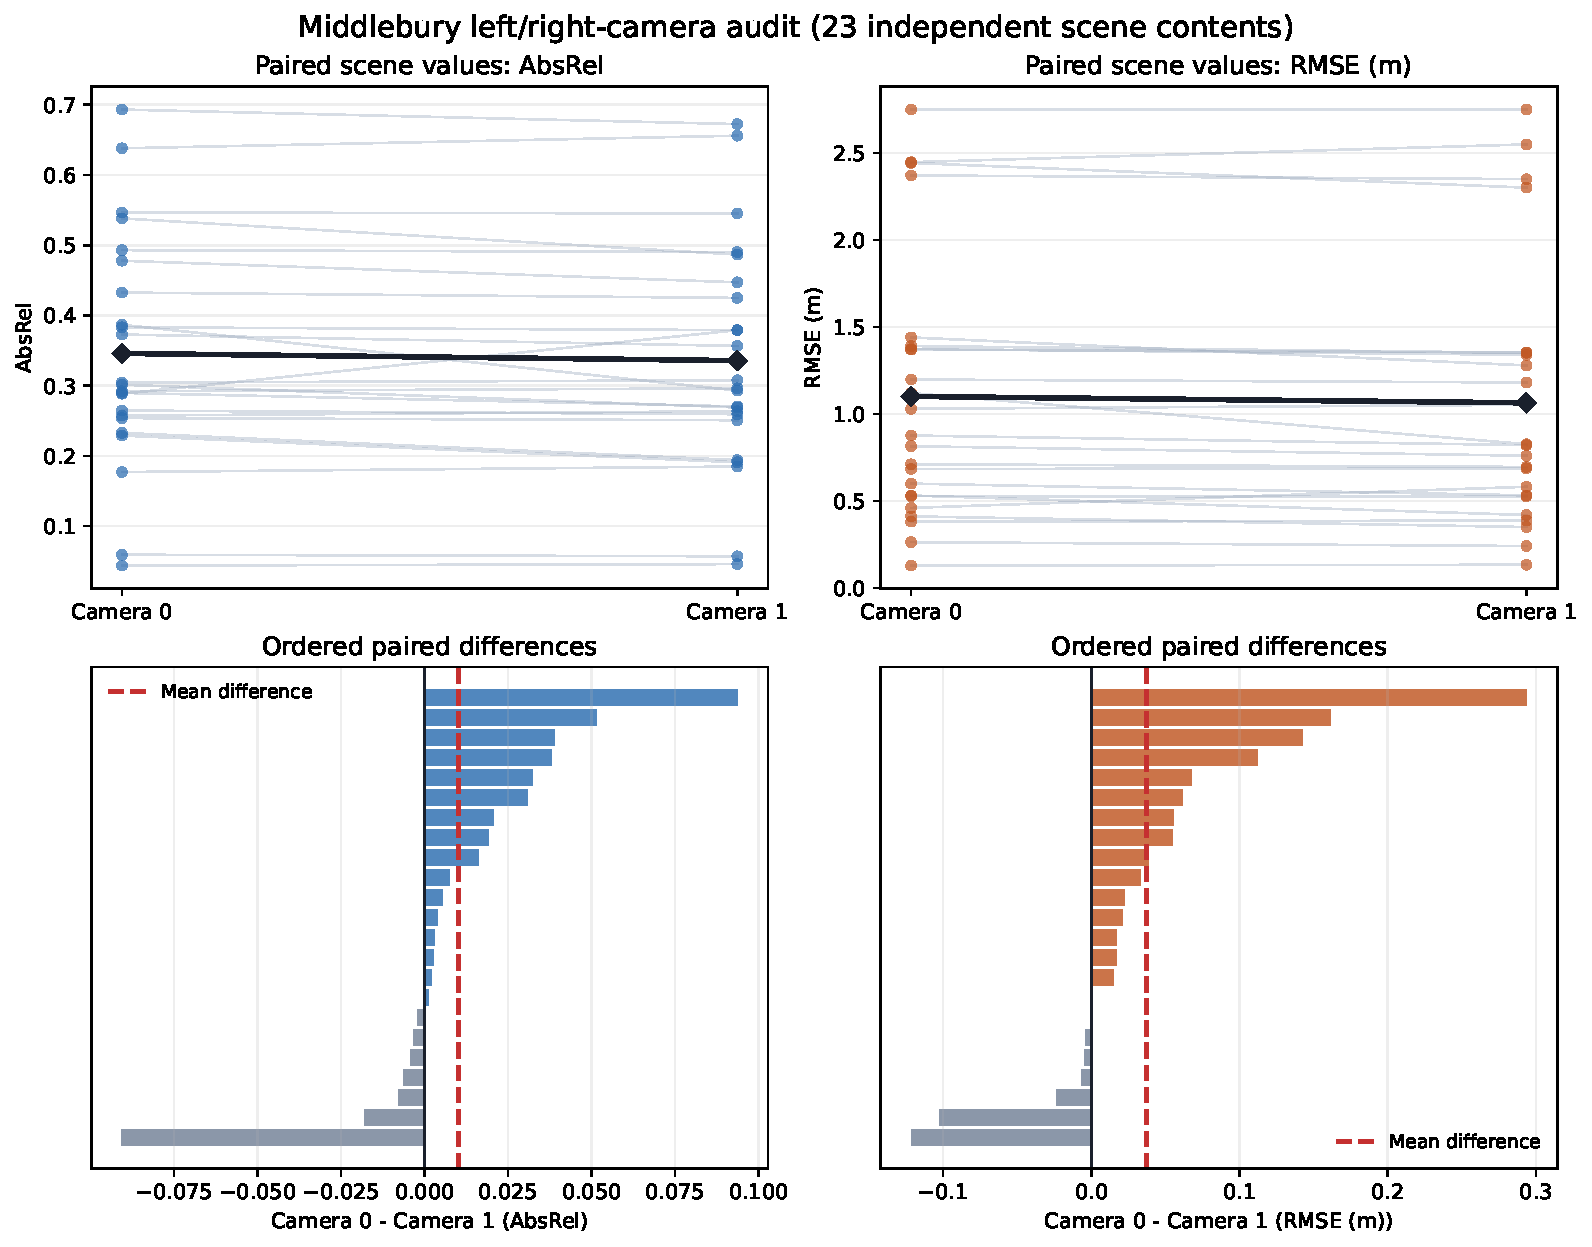
\includegraphics[width=0.98\textwidth]{./figures/middlebury_camera_audit.pdf}
    \caption{مقایسهٔ زوجی دو سمت دوربین در \lr{Middlebury} پس از میانگین‌گیری دو نسخهٔ تصحیح هر یک از ۲۳ محتوای صحنه. ردیف بالا مقادیر هر صحنه و میانگین کل (لوزی سیاه) و ردیف پایین اختلاف مرتب‌شدهٔ دوربین ۰ منهای دوربین ۱ را نشان می‌دهد. خط‌چین قرمز میانگین اختلاف است.}
    \label{fig:middlebury_camera_audit}
\end{figure}

این نتیجه از حساسیت بیشتر \lr{RMSE} به تفاوت نظام‌مند میان دو سمت تصویربرداری پشتیبانی می‌کند، اما به‌تنهایی اثر علّی یک مؤلفهٔ مشخص از $K$ را اثبات نمی‌کند؛ زیرا دو ورودی، دیدگاه و محتوای پیکسلی کاملاً یکسانی ندارند و \basemodel{} نیز $K$ را به‌صورت صریح دریافت نمی‌کند. شواهد علّی مصرف $K$ در فصل بعد با کنترل تصویر و تغییر مستقیم ورودی $K$ ارائه می‌شود.

\subsection{عدم کفایت رویکرد ضمنی نسبت به مشخصه‌های دوربین}

روش‌هایی که بدون لحاظ صریح ماتریس مشخصهٔ دوربین\enfootnote{Camera Intrinsic Matrix (\(K\))} توسعه یافته‌اند، اغلب متکی بر راهبردهای یادگیری روابط نسبی یا بازسازی بر مبنای هندسهٔ ضمنی هستند؛ به این معنا که مدل، صرفاً براساس روابط داخلی پیکسل‌های تصویر، بدون آگاهی از مقیاس مطلق صحنه یا فواصل کانونی واقعی، اقدام به بازسازی عمق می‌کند. این سیاست، علاوه بر ایجاد وابستگی پنهان مدل نسبت به توزیع دوربین‌های موجود در مرحلهٔ آموزش، در عمل منجر به آن می‌شود که مدل به محض مواجهه با تصاویر ثبت‌شده توسط دوربینی با پارامترهای متفاوت، دیگر قادر به تولید تخمین‌های متریک دقیق نیست.

این موضوع به‌ویژه در کاربردهای عملی، که تصاویر ورودی ممکن است مجموعه‌ای ناهمگن از لحاظ نوع، رزولوشن، و پارامترهای اپتیکی باشند، مصداق می‌یابد و موجب کاهش جدی قابلیت اعتماد مدل در محیط‌های واقعی می‌شود. افزون بر آن، تضعیف ارزیابی مدل با معیارهای متریک (همانند \lr{RMSE}) نه تنها مانعی برای ارتقاء کیفی سیستم‌های بینایی ماشینی محسوب می‌شود، بلکه حتی قابلیت رقابت مدل با سنسورهای عمق‌سنج فیزیکی را نیز با چالش جدی مواجه می‌سازد.

\subsection{کاربردهای عملی و انتقال‌پذیری به داده‌های جهان واقعی}

در بسیاری از کاربردهای کلیدی تخمین عمق تک‌دوربینه، از جمله رباتیک، هدایت خودکار وسایل نقلیه، نقشه‌برداری سه‌بعدی، و واقعیت افزوده، داده‌های تصویری از منابع و دوربین‌های متعددی تأمین می‌شوند که هریک دارای ویژگی‌های اپتیکی منحصربه‌فردی هستند. انتقال موفق مدل از شرایط آزمایشگاهی به محیط‌های عملی، مستلزم آن است که سامانه بتواند برای هر تصویر ورودی، با استفاده از ماتریس مشخصهٔ دوربین متناظر آن، عمل تخمین عمق را به‌صورت سازگار و قابل اطمینانی انجام دهد. پژوهش‌هایی که اخیراً حول موضوع جبران و بهبود رفتار مدل نسبت به زاویهٔ دید (FOV) و کالیبراسیون دوربین در مجموعه‌داده‌های مختلف منتشر شده است \cite{Saxena2023FOV}، بر همین نکته تأکید دارند: لحاظ صریح مشخصات دوربین، کلید دستیابی به یک تخمین عمق متریک باکیفیت و مقاوم در کاربردهای واقعی است.

\subsection{لزوم طراحی مدل با ورود صریح پارامترهای درونی}

برآیند این شواهد نظری و تجربی، این ضرورت را آشکار می‌کند که طراحی مدل‌هایی که به دنبال تخمین عمق متریک هستند، باید به‌طور ساختاری از اطلاعات پارامترهای دوربین (و به‌طور ویژه ماتریس $K$) بهره گیرند. لحاظ $K$، چه به‌صورت ورودی صریح به شبکه، چه از طریق تطبیق ساختار لایه‌های مدل با قیود فیزیکی تصویربرداری، می‌تواند پایداری و دقت تخمین عمق را در مواجهه با تنوع عملی داده‌ها تضمین کند.  

رویکرد پیشنهادی ما در این پژوهش، مبتنی بر ورود ساخت‌یافتهٔ اطلاعات ماتریس مشخصهٔ دوربین در جریان یادگیری و استنتاج مدل است؛ رویکردی که شواهد ریاضی و تجربی، برتری آن را به‌ویژه در ارزیابی عمق متریک ثابت کرده‌اند. جزییات پیاده‌سازی این ایده و ادغام $K$ با معماری پایه، در بخش‌های بعدی ارائه خواهد شد.

% sec 6
\section{طراحی روش پیشنهادی: ادغام صریح ماتریس مشخصهٔ دوربین}

بر اساس مباحث نظری ارائه‌شده در بخش‌های پیشین و شواهد تجربی حاصل از تحلیل حساسیت معیارهای متریک نسبت به پارامترهای درونی دوربین، در این پژوهش روشی برای ادغام صریح ماتریس مشخصهٔ دوربین در معماری \lr{Depth Anything V2} پیشنهاد می‌شود. ایدهٔ اصلی این روش، فراهم‌کردن امکان دسترسی مستقیم مدل به اطلاعات هندسی فرآیند تصویربرداری است، به‌گونه‌ای که شبکه به‌جای استنتاج ضمنی و ناپایدار این اطلاعات از روی داده، بتواند از قیود فیزیکی دوربین به‌صورت ساخت‌یافته بهره‌مند شود\cite{Zhou2017Unsupervised, Ranftl2019Robust}.


در این بخش، ابتدا اصول کلی طراحی روش پیشنهادی تشریح می‌شود، سپس نحوهٔ نمایش و نرمال‌سازی ماتریس مشخصهٔ دوربین توضیح داده شده و در ادامه، راهبرد ادغام این اطلاعات با معماری encoder--decoder \basemodel{} مورد بررسی قرار می‌گیرد.

\subsection{اصل طراحی: تفکیک اطلاعات تصویری و هندسی}

در اغلب مدل‌های تخمین عمق تک‌دوربینه بدون نظارت، تصویر ورودی تنها منبع اطلاعاتی شبکه محسوب می‌شود و تمام قیود هندسی، اعم از فاصلهٔ کانونی یا میدان دید، به‌صورت ضمنی در وزن‌های مدل جذب می‌شوند\cite{Godard2019Digging, Ranftl2021DPT}. این رویکرد باعث می‌شود که مدل به توزیع دوربین‌های موجود در دادهٔ آموزشی وابسته شود و در مواجهه با داده‌هایی که از نظر پارامترهای درونی تفاوت دارند، عملکرد ناپایداری از خود نشان دهد.

روش پیشنهادی این پژوهش بر اصل تفکیک میان اطلاعات تصویری و اطلاعات هندسی استوار است. در این چارچوب، تصویر ورودی همچنان به‌عنوان منبع اطلاعات ظاهری و معنایی صحنه مورد استفاده قرار می‌گیرد، در حالی که ماتریس مشخصهٔ دوربین به‌عنوان توصیف‌گر هندسهٔ تصویربرداری، به‌صورت یک ورودی مستقل و مکمل در اختیار مدل قرار داده می‌شود. این تفکیک، به مدل اجازه می‌دهد تا نگاشت میان پیکسل و عمق را نه‌تنها بر اساس الگوهای بصری، بلکه با در نظر گرفتن مقیاس و هندسهٔ واقعی دوربین   انجام دهد \cite{Casser2019DepthSensors, Sucar2020ImplicitGeometry}.

\subsection{نمایش و پیش‌پردازش ماتریس مشخصهٔ دوربین}

ماتریس مشخصهٔ دوربین به‌صورت زیر تعریف می‌شود:
\begin{equation}
K =
\begin{bmatrix}
f_x & 0   & c_x \\
0   & f_y & c_y \\
0   & 0   & 1
\end{bmatrix}.
\end{equation}

از آنجا که مقادیر این ماتریس به رزولوشن تصویر و تنظیمات فیزیکی دوربین وابسته‌اند، استفادهٔ مستقیم از مقادیر خام می‌تواند موجب ناپایداری عددی در فرآیند یادگیری شود \cite{Kendall2015GeometryAware, Zhou2017Unsupervised}. به همین دلیل، در روش پیشنهادی، پارامترهای درونی دوربین پیش از ورود به شبکه نرمال‌سازی می‌شوند. به‌طور خاص، مؤلفه‌های فاصلهٔ کانونی و مختصات نقطهٔ اصلی بر حسب ابعاد تصویری که ماتریس $K$ در آن بیان شده است نرمال می‌شوند:
\begin{equation}
\tilde{f}_x = \frac{f_x}{W}, \quad
\tilde{f}_y = \frac{f_y}{H}, \quad
\tilde{c}_x = \frac{c_x}{W}, \quad
\tilde{c}_y = \frac{c_y}{H},
\end{equation}
که در آن $W$ و $H$ به‌ترتیب عرض و ارتفاع چارچوب مرجع پارامترهای دوربین هستند. این بازنمایی نرمال‌شده، امکان استفادهٔ پایدار از اطلاعات دوربین در مجموعه‌داده‌هایی با رزولوشن‌های متفاوت را فراهم می‌کند \cite{Chen2022CameraAware, Guizilini2020SemanticallyGuided}.

افزون بر مؤلفه‌های نرمال‌شدهٔ فوق، برای آنکه بازنمایی ورودی به‌صورت مستقیم دربردارندهٔ مفهوم فیزیکی میدان دید\enfootnote{Field of View (FoV)} باشد، زوایای میدان دید افقی و عمودی نیز به‌صورت
\begin{equation}
\mathrm{fov}_w = 2\,\arctan\!\left(\frac{W}{2 f_x}\right), \qquad
\mathrm{fov}_h = 2\,\arctan\!\left(\frac{H}{2 f_y}\right)
\end{equation}
محاسبه می‌شوند. مطابق پیاده‌سازی نهایی، زاویه‌ها بر $\pi$، میانگین فاصلهٔ کانونی بر بزرگ‌ترین بُعد تصویر و مساحت تصویر بر مساحت مرجع $1920\times1080$ تقسیم می‌شوند. بنابراین، بردار توصیف‌گر هندسی دوربین دقیقاً به‌صورت
\begin{equation}
\mathbf{k} = \left[\frac{f_x}{W},\;\frac{f_y}{H},\;\frac{c_x}{W},\;\frac{c_y}{H},\;
\frac{\mathrm{fov}_h}{\pi},\;\frac{\mathrm{fov}_w}{\pi},\;\frac{W}{H},\;
\frac{f_x+f_y}{2\max(H,W)},\;\frac{HW}{1920\times1080}\right]
\end{equation}
تعریف می‌شود و به‌عنوان ورودی هندسی مدل مورد استفاده قرار می‌گیرد. نکتهٔ اساسی در این بازنمایی آن است که ماتریس $K$ و ابعاد $(H, W)$ باید هر دو در یک چارچوب مختصات یکسان بیان شوند؛ در غیر این صورت، کدگذاری حاصل از منظر هندسی نادرست خواهد بود. اهمیت عملی این نکته در بخش جزئیات پیاده‌سازی و در تحلیل اشکال‌زدایی فصل چهارم آشکار می‌شود.

\subsection{راهبرد ادغام اطلاعات دوربین با معماری \lr{Depth Anything V2}}

برای ادغام بردار پارامترهای درونی دوربین با معماری پایه، در این پژوهش از یک واحد کدگذار دوربین\enfootnote{Camera Encoder} استفاده می‌شود که وظیفهٔ آن، تبدیل بردار کم‌بعد $\mathbf{k}$ به یک \emph{توکن دوربین} سازگار با فضای بازنمایی ترنسفورمر است. این واحد شامل یک شبکهٔ تمام‌متصل دولایه برای نگاشت اولیه و سپس چند بلوک ترنسفورمر برای پالایش بازنمایی است که خروجی آن یک توکن با ابعاد برابر با بعد نهان انکودر بینایی است:
\begin{equation}
\mathbf{z}_k = \phi(\mathbf{k}),
\end{equation}
که در آن $\phi(\cdot)$ تابع نگاشت پارامتری قابل یادگیری است.

توکن دوربین $\mathbf{z}_k$ سپس در کنار توکن‌های تصویری، به دنبالهٔ توکن‌های انکودر مبتنی بر \lr{DINOv2} تزریق می‌شود؛ به‌گونه‌ای که سازوکار خودتوجهی بتواند در تمامی لایه‌های پس از نقطهٔ تزریق، اطلاعات هندسی دوربین را با بازنمایی‌های بصری ترکیب کند. لایهٔ تزریق از طریق پارامتر قابل تنظیم
\lr{\texttt{-{}-cam-\allowbreak token-\allowbreak inject-\allowbreak layer}}
کنترل می‌شود و در تنظیمات پیش‌فرض، تزریق از نخستین لایهٔ انکودر انجام می‌گیرد. این راهبرد با روش‌های شرطی‌سازی مبتنی بر توکن در معماری‌های ترنسفورمری و نیز رویکردهای تنظیم ویژگی به‌کمک بردارهای شرطی نظیر FiLM هم‌خانواده است \cite{Perez2018FiLM}؛ با این تفاوت که در اینجا، شرطی‌سازی از طریق سازوکار توجه انجام می‌شود و نیازی به دستکاری مستقیم نگاشت‌های ویژگی نیست.

نکتهٔ طراحی مهم در این ادغام، استفاده از یک \emph{دروازهٔ خروجی با مقداردهی اولیهٔ صفر}\enfootnote{Zero-initialized Output Gate} است: خروجی کدگذار دوربین در ابتدای آموزش در یک ضریب قابل یادگیری با مقدار اولیهٔ صفر ضرب می‌شود. در نتیجه، در گام‌های نخست آموزش، توکن دوربین عملاً برداری صفر است و رفتار مدل دقیقاً با مدل ازپیش‌آموزش‌دیدهٔ پایه یکسان باقی می‌ماند؛ سپس در طول آموزش، شبکه به‌تدریج و تنها در صورتی که اطلاعات دوربین برای کاهش خطا مفید باشد، این دروازه را باز می‌کند. این سازوکار، از آسیب رساندن به بازنمایی‌های ازپیش‌آموخته در آغاز فاین‌تیون جلوگیری کرده و پایداری فرآیند آموزش را تضمین می‌کند \cite{Casser2019DepthSensors, Li2021NeuralSceneFlow}.

\begin{figure}[htbp]
    \centering
    \resizebox{\textwidth}{!}{%
    \begin{tikzpicture}[
        node distance=0.8cm and 1cm,
        block/.style={draw, thick, fill=blue!10, rectangle, minimum height=1cm, minimum width=2.5cm, align=center, rounded corners},
        data/.style={draw, thick, fill=green!10, ellipse, align=center},
        arrow/.style={thick, -Latex}
    ]
    
    % Input
    \node[data] (img) {تصویر ورودی $I$};
    \node[data, below=2cm of img] (intrinsics) {ماتریس مشخصه $K$};
    
    % Models
    \node[block, right=of img, fill=red!10] (encoder) {انکودر (DINOv2) \\ \small (ویژگی‌های چندمقیاسی)};
    \node[block, right=of intrinsics, fill=orange!10] (k_encoder) {کدگذار دوربین \\ \small (MLP)};
    
    % Latent
    \node[data, right=of k_encoder] (z_k) {توکن دوربین $\mathbf{z}_k$};
    
    % Decoder
    \node[block, right=of encoder, minimum height=2.5cm] (decoder) {دیکودر (DPT) \\ \small (بازیابی رزولوشن و عمق)};
    
    % Output
    \node[data, right=of decoder] (depth) {عمق متریک $D$};
    
    % Connections
    \draw[arrow] (img) -- (encoder);
    \draw[arrow] (intrinsics) -- (k_encoder);
    \draw[arrow] (k_encoder) -- (z_k);
    \draw[arrow] (encoder) -- (decoder) node[midway, above] {ویژگی‌ها};

    \draw[arrow, dashed, thick] (z_k) |- (encoder.south east) node[pos=0.35, right] {تزریق توکن دوربین};
    \draw[arrow] (decoder) -- (depth);

    \end{tikzpicture}%
    }
    \caption{معماری \proposedmodel{}: اطلاعات تصویر توسط انکودر ازپیش‌آموزش‌دیده استخراج می‌شود. ماتریس مشخصهٔ دوربین $K$ پس از نرمال‌سازی، توسط واحد کدگذار دوربین به یک توکن نهان تبدیل شده و همراه با یک دروازهٔ خروجی صفرمقدار اولیه، به دنبالهٔ توکن‌های انکودر تزریق می‌گردد تا سازوکار توجه بتواند اطلاعات هندسی را با بازنمایی‌های بصری ترکیب کند.}
    \label{fig:proposed_architecture}
\end{figure}

\subsection{مزایای مورد انتظار از ادغام صریح پارامترهای درونی}

ادغام صریح ماتریس مشخصهٔ دوربین، چند مزیت کلیدی را به همراه دارد. نخست آنکه مدل قادر خواهد بود نگاشت میان پیکسل و عمق را با در نظر گرفتن مقیاس واقعی دوربین انجام دهد و از این طریق، دقت تخمین عمق متریک افزایش یابد. دوم آنکه وابستگی مدل به توزیع خاصی از دوربین‌ها در دادهٔ آموزشی کاهش می‌یابد و تعمیم‌پذیری آن در مواجهه با داده‌های چنددوربینه بهبود پیدا می‌کند. این موضوع به‌ویژه با توجه به نتایج تجربی ارائه‌شده در تحلیل RMSE در بخش پیشین، اهمیت ویژه‌ای دارد. در نهایت، این طراحی امکان توسعهٔ مدل به سناریوهای پیشرفته‌تر، نظیر یادگیری انتقالی میان مجموعه‌داده‌های با میدان دید متفاوت، را نیز فراهم می‌کند.

در بخش‌های بعدی، نحوهٔ آموزش این مدل، تابع هزینهٔ مورد استفاده، و تنظیمات تجربی برای ارزیابی اثر ادغام پارامترهای درونی دوربین به‌تفصیل تشریح خواهد شد.

% sec 7
 \section{راهبرد آموزش \proposedmodel{}}

در این پژوهش، آموزش \proposedmodel{} به‌صورت فاین‌تیون\enfootnote{Fine-tuning} یک مدل ازپیش‌آموزش‌یافته انجام شده است. به‌طور خاص، از \basemodel{}، نسخهٔ غیرمتریک با وزن‌های اولیهٔ مدل Large به‌عنوان نقطهٔ شروع استفاده شده و فرآیند آموزش با هدف تبدیل آن به یک مدل متریک پایدار، با لحاظ صریح پارامترهای درونی دوربین، طراحی شده است. این راهبرد، ضمن بهره‌گیری از دانش غنی مدل معلم، امکان انطباق مدل با تنظیمات هندسی جدید را بدون نیاز به آموزش از ابتدا فراهم می‌کند.

برای رفع ابهام اصطلاح‌شناختی، عنوان کلی پژوهش به تخمین عمق بدون نظارت و استفاده از یک مدل بنیادین ازپیش‌آموخته اشاره دارد، اما مرحلهٔ نهایی فاین‌تیون کنترل‌شده در این پایان‌نامه \emph{نظارتی} است و از نگاشت‌های عمق مرجع \lr{NYUv2} استفاده می‌کند. تقطیر دانش در زیرساخت پیاده‌سازی شده، ولی در آزمایش‌های نهایی غیرفعال است. این تفکیک ضروری است تا بهبود مشاهده‌شده به ورودی $K$ و برنامهٔ فاین‌تیون نسبت داده شود، نه به یک سیگنال آموزشی جانبی.

\subsection{مجموعه‌داده‌های مورد استفاده}

در مرحلهٔ اکتشافی، ترکیب‌هایی از \lr{Virtual KITTI}\enfootnote{Virtual KITTI}، \lr{NYUv2}\enfootnote{NYUv2}، \lr{DIODE}\enfootnote{DIODE}، \lr{Cityscapes} و \lr{Middlebury} آزموده شد. این داده‌ها از نظر نوع صحنه، شرایط تصویربرداری و مشخصات دوربین متنوع‌اند \cite{Gaidon2016VKITTI, Silberman2012NYUv2, Vasiljevic2019DIODE}؛ بااین‌حال، نتایج فصل چهارم نشان داد که فاین‌تیون چندمجموعه‌ای محدود، تعمیم صفرنمونهٔ مدل بنیادین را تخریب می‌کند. ازاین‌رو، مطالعهٔ نهایی برای جداسازی علّی سهم $K$ به \lr{NYUv2} محدود شد و هر زوج \proposedmodel{}/\controlmodel{} دقیقاً داده‌ها و برنامهٔ آموزشی یکسانی دریافت کرد.

داده‌های مورد استفاده عمدتاً به‌صورت تک‌تصویر یا توالی‌های کوتاه از تصاویر ثبت‌شده‌اند، با این تفاوت که در فرآیند آموزش حاضر، هر تصویر به‌صورت مستقل پردازش شده و هیچ‌گونه قید زمانی یا وابستگی صریح میان فریم‌های متوالی اعمال نشده است. این انتخاب، با هدف تمرکز بر مسئلهٔ تخمین عمق تک‌تصویر و حذف اثرات جانبی ناشی از حرکت دوربین یا برآورد ژست صورت گرفته است.

در مواردی که اطلاعات ماتریس مشخصهٔ دوربین به‌صورت صریح در داده‌ها موجود بوده، این اطلاعات مستقیماً مورد استفاده قرار گرفته و در سایر موارد، پارامترهای دوربین مطابق با تنظیمات مرجع هر مجموعه‌داده استخراج یا بازسازی شده‌اند.

\subsection{تفکیک صحیح مجموعه‌های آموزش و آزمون در NYUv2}

نکتهٔ روش‌شناختی مهمی که در جریان این پژوهش شناسایی و اصلاح شد، نحوهٔ تفکیک داده‌های آموزش و آزمون در مجموعه‌دادهٔ \lr{NYUv2} است. پروتکل استاندارد ارزیابی در ادبیات این حوزه، زیرمجموعهٔ آزمون ۶۵۴ تصویری موسوم به تقسیم‌بندی \lr{Eigen} است \cite{Eigen2014Depth} که مدل \lr{Depth Anything V2} نیز نتایج خود را بر همین مبنا گزارش می‌کند \cite{DepthAnythingV2}. در نسخهٔ اولیهٔ زیرساخت آموزش این پژوهش، تقسیم‌بندی آموزش/اعتبارسنجی به‌صورت تصادفی بر روی کل ۱۴۴۹ تصویر مجموعهٔ برچسب‌دار انجام می‌شد؛ بررسی دقیق نشان داد که با این رویه، ۵۲۷ تصویر از ۶۵۴ تصویر آزمون استاندارد (معادل \fadecimal{۸۰٫۶} درصد) در مجموعهٔ آموزش قرار می‌گیرند و در نتیجه هرگونه ارزیابی روی مجموعهٔ آزمون، دچار نشت داده\enfootnote{Data Leakage} و به‌صورت مصنوعی خوش‌بینانه خواهد بود.

برای رفع این مشکل، فرآیند تقسیم‌بندی به‌گونه‌ای اصلاح شد که ابتدا تمامی ۶۵۴ تصویر آزمون استاندارد به‌طور کامل کنار گذاشته شوند و سپس تقسیم ۸۰/۲۰ آموزش/اعتبارسنجی تنها بر روی ۷۹۵ تصویر باقی‌مانده انجام گیرد (۶۳۶ تصویر آموزش و ۱۵۹ تصویر اعتبارسنجی). عدم هم‌پوشانی سه مجموعه نیز با آزمون خودکار راستی‌آزمایی شده است. تمامی نتایج نهایی گزارش‌شده در فصل چهارم بر مبنای این تفکیک بدون نشت به‌دست آمده‌اند.

\subsection{\basemodel{} و راهبرد فاین‌تیون}

نسخهٔ غیرمتریک \basemodel{} به‌صورت teacher–student distillation\enfootnote{Teacher–Student Distillation} آموزش دیده و دارای توانایی بالایی در استخراج ویژگی‌های معنایی و هندسی تصویر است. در این پژوهش، این مدل به‌عنوان دانش اولیه در نظر گرفته شده و فرآیند فاین‌تیون با هدف افزودن قابلیت تخمین عمق متریک و تطبیق با اطلاعات دوربین انجام شده است.

برای حفظ پایداری آموزش و جلوگیری از بیش‌برازش، بخش encoder مبتنی بر \lr{DINOv2}\enfootnote{DINOv2} در طول آموزش فریز شده است. این تصمیم مبتنی بر این فرض است که ویژگی‌های استخراج‌شده توسط \lr{DINOv2}، پیشاپیش از غنای کافی برای نمایش محتوای تصویری برخوردارند و نیازی به بازآموزی در این مرحله ندارند \cite{Oquab2023DINOv2}. در مقابل، بخش decoder و همچنین ماژول‌های مرتبط با تخمین عمق و پردازش پارامترهای دوربین، به‌صورت کامل قابل یادگیری باقی مانده‌اند.

\subsection{فعال‌سازی پشتیبانی از پارامترهای دوربین}

گزینهٔ \lr{\texttt{-{}-use-camera-intrinsics}} در اسکریپت آموزش، استفاده از ماتریس مشخصهٔ دوربین را در فرآیند آموزش فعال می‌کند. با فعال‌سازی این گزینه، بردار نرمال‌سازی‌شدهٔ پارامترهای دوربین مطابق با توضیحات بخش ۳–۶ استخراج شده و از طریق یک encoder اختصاصی به فضای نهان مدل نگاشت می‌شود.

علاوه بر این، امکان کنترل محل تزریق اطلاعات دوربین در معماری شبکه از طریق پارامتر \lr{\texttt{-{}-cam-\allowbreak token-\allowbreak inject-\allowbreak layer}} فراهم شده است. این پارامتر لایهٔ تزریق توکن به \emph{انکودر} \lr{DINOv2} را تعیین می‌کند. در تمام آزمایش‌های گزارش‌شده مقدار پیش‌فرض، یعنی لایهٔ نخست انکودر، استفاده شده است؛ حساسیت نسبت به محل تزریق و تزریق چندلایه در این پژوهش پیمایش نشده و به‌عنوان مسیر کار آینده گزارش می‌شود.

\subsection{تنظیمات آموزش و بهینه‌سازی}

فرآیند آموزش با اسکریپت \lr{\texttt{train.py}} و در دو حالت انجام شده است: \lr{\texttt{-{}-model-type basic}} برای خروجی نسبی در فضای عمق معکوس، و \lr{\texttt{-{}-model-type metric}} برای عمق مطلق بر حسب متر. حالت نسبی برای بازتولید پروتکل استاندارد و تشخیص محدودیت تراز مقیاس به‌کار رفت؛ حالت متریک، بستر اصلی آزمون فرضیهٔ نقش $K$ در بازیابی مقیاس بود.

به‌منظور سازگاری بهتر فرآیند فاین‌تیون با وزن‌های ازپیش‌آموزش‌یافته، نرخ یادگیری بخش‌های مختلف شبکه به‌صورت ناهمسان تنظیم شده است. به‌طور خاص، برای لایه‌های مربوط به تخمین عمق و encoder پارامترهای دوربین، از ضریب تقویت نرخ یادگیری استفاده شده است:
\begin{equation}
\texttt{\lr{--head-lr-multiplier}}
\end{equation}
این راهبرد باعث می‌شود که لایه‌های جدید یا تغییر یافته، سریع‌تر با هدف متریک آموزش تطبیق یابند، در حالی که سایر بخش‌های شبکه دچار نوسان شدید نشوند.

همچنین، برای افزایش پایداری عددی آموزش، از برش گرادیان\enfootnote{Gradient Clipping} و در برخی تنظیمات از warm-up تدریجی نرخ یادگیری استفاده شده است. این تنظیمات به‌ویژه در مراحل ابتدایی آموزش، از واگرایی گرادیان‌ها جلوگیری کرده و همگرایی نرم‌تری را فراهم می‌کنند.

\subsection{فضای هدف آموزش برای مدل‌های نسبی: عمق معکوس}
\label{subsec:disparity_target_space}

یکی از یافته‌های روش‌شناختی مهم این پژوهش، اهمیت \emph{هم‌خوانی فضای هدف آموزش با فضای خروجی مدل ازپیش‌آموزش‌دیده} است. \basemodel{}، نسخهٔ نسبی، مطابق با سنت روش‌های خانوادهٔ \lr{MiDaS} \cite{Ranftl2019Robust}، در فضای \emph{عمق معکوس} (دیسپاریتی)\enfootnote{Inverse Depth / Disparity} آموزش دیده و خروجی آن با عمق رابطهٔ وارون دارد: نقاط نزدیک مقادیر بزرگ و نقاط دور مقادیر کوچک دریافت می‌کنند.

در نسخهٔ اولیهٔ زیرساخت آموزش این پژوهش، مقادیر عمق مستقیم به‌عنوان هدف آموزشی مدل نسبی به‌کار می‌رفت. تحلیل دقیق این تنظیم نشان داد که ترکیب آن با تابع هزینهٔ تغییرناپذیر نسبت به مقیاس و جابجایی، به یک شکست خاموش\enfootnote{Silent Failure} منجر می‌شود: از یک سو، محدودسازی ضریب مقیاس $s$ به مقادیر مثبت در پیاده‌سازی تابع هزینه، برازش رابطهٔ وارون میان خروجی دیسپاریتی و هدف عمق مستقیم را ناممکن می‌سازد؛ و از سوی دیگر، مؤلفهٔ تطابق گرادیان که بر روی مقادیر تراز‌نشده محاسبه می‌شود، دامنهٔ خروجی مدل را به‌شدت به سمت صفر سوق می‌دهد. برآیند این دو عامل آن است که بهینهٔ عملی تابع هزینه، خروجی ثابت صفر است و تابع فعال‌سازی \lr{ReLU} در انتهای سر شبکه، این حالت را برگشت‌ناپذیر می‌کند (گرادیان صفر). آزمایش کنترل‌شدهٔ ابزارگذاری‌شده نشان داد که مدل \lr{ViT-L} تنها در حدود ۱۸ گام آموزشی به‌طور کامل به این حالت فرو می‌ریزد؛ این در حالی است که منحنی هزینهٔ آموزش ظاهری کاملاً طبیعی دارد، زیرا با خروجی ثابت، مقدار هزینه صرفاً تابع آماره‌های داده در هر دسته است. جزئیات تجربی این پدیده و فرآیند تشخیص آن در فصل چهارم گزارش شده است.

بر این اساس، در چارچوب نهایی آموزش، هدف مدل‌های نسبی به فضای عمق معکوس منتقل شد:
\begin{equation}
T_{\mathrm{disp}} = \frac{1}{\max(D^{GT}, d_{\min})},
\end{equation}
که در آن $d_{\min}$ کران پایین عمق معتبر است. با این تغییر، فضای هدف با فضای خروجی مدل ازپیش‌آموزش‌دیده هم‌راستا شده و فرآیند فاین‌تیون بدون فروریزش و با پایداری کامل انجام می‌گیرد. متناظر با آن، ارزیابی اعتبارسنجی حین آموزش نیز با ترازکردن مقیاس و جابجایی در فضای عمق معکوس و سپس وارون‌سازی به فضای عمق انجام می‌شود و نوع فضای هدف در فراداده‌های ذخیره‌شدهٔ هر نقطهٔ وارسی\enfootnote{Checkpoint} ثبت می‌گردد تا زنجیرهٔ ارزیابی به‌صورت خودکار رفتار صحیح را اتخاذ کند.

\subsection{افزونه‌سازی هندسی آگاه از پارامترهای دوربین}
\label{subsec:fov_augmentation}

چالش بنیادی در آموزش \proposedmodel{} بر روی یک مجموعه‌دادهٔ تک‌دوربینه (نظیر \lr{NYUv2} که تمامی تصاویر آن با یک حسگر \lr{Kinect} ثبت شده‌اند) آن است که بردار $\mathbf{k}$ برای تمامی نمونه‌ها ثابت است و در نتیجه هیچ سیگنال تمایزبخشی برای واحد کدگذار دوربین فراهم نمی‌کند. افزون بر این، بررسی زیرساخت اولیهٔ آموزش نشان داد که برش تصادفی\enfootnote{Random Crop} متداول در خط لولهٔ پیش‌پردازش، مرکز تصویر مؤثر را جابه‌جا می‌کند بدون آنکه ماتریس $K$ متناظراً به‌روزرسانی شود؛ در نتیجه، کدگذار دوربین در عمل اطلاعاتی \emph{ثابت و از منظر هندسی نادرست} دریافت می‌کرد.

برای رفع هم‌زمان هر دو مشکل، در این پژوهش یک راهبرد افزونه‌سازی هندسی دقیق طراحی و پیاده‌سازی شد که در آن، برای هر نمونهٔ آموزشی، پنجره‌ای تصادفی با نسبت ابعادی ثابت ۴:۳ و ضریب بزرگ‌نمایی $s$ (در بازهٔ ۱ تا حداکثر \fadecimal{۱٫۷} یا \fadecimal{۲٫۲} بسته به تنظیم آزمایش، و با احتمال ۲۰ درصد دقیقاً قاب کامل) از تصویر بریده می‌شود و ماتریس $K$ به‌صورت \emph{دقیق} در تمامی مراحل هندسی به‌روزرسانی می‌گردد: جابه‌جایی نقطهٔ اصلی متناسب با مبدأ پنجرهٔ برش،
\begin{equation}
c_x' = c_x - x_0, \qquad c_y' = c_y - y_0,
\end{equation}
و مقیاس‌دهی فاصلهٔ کانونی و نقطهٔ اصلی متناسب با تغییر اندازهٔ پنجره به چارچوب ثابت ورودی شبکه:
\begin{equation}
\begin{aligned}
f_x' &= f_x \frac{W_{\mathrm{net}}}{w_{\mathrm{win}}}, &
c_x' &= (c_x-x_0)\frac{W_{\mathrm{net}}}{w_{\mathrm{win}}},\\
f_y' &= f_y \frac{H_{\mathrm{net}}}{h_{\mathrm{win}}}, &
c_y' &= (c_y-y_0)\frac{H_{\mathrm{net}}}{h_{\mathrm{win}}}.
\end{aligned}
\end{equation}
که در آن $(H_{\mathrm{net}}, W_{\mathrm{net}})$ ابعاد ثابت چارچوب ورودی شبکه (در پیاده‌سازی حاضر $518 \times 686$، مضرب اندازهٔ وصله‌های ترنسفورمر) است. مقادیر عمق در این تبدیل تغییر نمی‌کنند، زیرا نقاط صحنه همان نقاط پیشین هستند.

وارونه‌سازی افقی نیز هم‌زمان بر تصویر، نگاشت عمق، ماسک اعتبار و ماتریس مشخصه اعمال می‌شود. در این حالت، مختصهٔ افقی نقطهٔ اصلی مطابق $c_x'=W-c_x$ اصلاح می‌گردد. همچنین ابعاد چارچوبی که $K$ در آن تعریف شده است همراه هر نمونه نگهداری می‌شود تا نرمال‌سازی مؤلفه‌های دوربین در آموزش و استنتاج دقیقاً در یک دستگاه مختصات انجام شود. این کنترل‌ها ضروری‌اند، زیرا تغییر تصویر بدون تبدیل متناظر $K$، حتی در صورت اجرای بی‌خطای برنامه، ورودی هندسی ناسازگار تولید می‌کند.

از منظر هندسی، این افزونه‌سازی معادل شبیه‌سازی دوربین‌هایی با میدان دید متفاوت از یک صحنهٔ واحد است: بزرگ‌نمایی $s$ میدان دید مؤثر را از حدود ۶۳ درجه (قاب کامل \lr{NYUv2}) تا حدود ۳۳ درجه تغییر می‌دهد. بدین ترتیب، \proposedmodel{} در طول آموزش با زوج‌های (تصویر، $K$) مواجه می‌شود که در آن‌ها ابهام میان مقیاس صحنه و میدان دید به‌صورت واقعی وجود دارد و تنها از طریق اطلاعات $K$ قابل رفع است؛ در حالی که \controlmodel{}، دقیقاً همین تصاویر افزونه‌سازی‌شده را بدون اطلاعات $K$ دریافت می‌کند. این طراحی، مبنای مطالعهٔ کنترل‌شدهٔ فصل چهارم برای سنجش سهم واقعی پارامترهای درونی دوربین است.

\subsection{افزونه‌سازی لرزش کانونی: غیرقابل‌حل‌کردن مقیاس بدون $K$}
\label{subsec:focal_jitter}

افزونه‌سازی زوم‌ـ‌برش زیربخش قبل، میدان دید را متنوع می‌کند، اما یک محدودیت بنیادی دارد: در تصاویر معمولی، نشانه‌های معنایی صحنه (ابعاد آشنای اشیاء، مبلمان، درها) به‌تنهایی برای بازیابی مقیاس تقریبی کافی‌اند و شبکه می‌تواند بدون مراجعه به $K$ نیز پاسخ قابل قبولی بدهد. برای آنکه اتکای مدل به پارامترهای درونی دوربین به یک \emph{ضرورت} تبدیل شود، در این پژوهش افزونه‌سازی مکملی با عنوان «لرزش کانونی»\enfootnote{Focal Jitter} طراحی شد که مستقیماً از معادلهٔ تصویربرداری روزنه‌ای الهام می‌گیرد. طبق این معادله، $u = f \cdot X / Z$، اگر فاصلهٔ کانونی در ضریب $\alpha$ و هم‌زمان تمام عمق‌های صحنه نیز در همان $\alpha$ ضرب شوند، تصویر حاصل \emph{دقیقاً یکسان} باقی می‌ماند. بر همین اساس، برای هر نمونهٔ آموزشی ضریبی به‌صورت لگاریتمی‌ـ‌یکنواخت از بازهٔ
\begin{equation}
\alpha \sim \exp\bigl(\mathcal{U}(-\ln m, +\ln m)\bigr), \qquad m = 1.6,
\end{equation}
نمونه‌برداری شده و تبدیل
\begin{equation}
f_x \mapsto \alpha f_x, \qquad f_y \mapsto \alpha f_y, \qquad Z \mapsto \alpha Z
\end{equation}
اعمال می‌شود؛ پیکسل‌های تصویر و مختصات نقطهٔ اصلی $(c_x, c_y)$ دست‌نخورده می‌مانند. این تبدیل از منظر هندسی \emph{دقیق} است (برخلاف بازنمونه‌برداری، هیچ خطای درون‌یابی ایجاد نمی‌کند) و هیچ نشتی اطلاعاتی ندارد، زیرا تصویر ورودی تغییری نمی‌کند.

پیامد این طراحی برای دو بازوی مطالعهٔ کنترل‌شده متقارن نیست: \controlmodel{} با تصاویری مواجه می‌شود که پیکسل‌های یکسان دارند اما برچسب‌های عمق متناقض؛ بهترین کاری که از آن برمی‌آید رگرسیون به میانگین توزیع $\alpha$ است و بخشی از خطا برای آن \emph{کاهش‌ناپذیر} می‌شود. در مقابل، \proposedmodel{} می‌تواند $\alpha$ را مستقیماً از مقدار فاصلهٔ کانونی بخواند و ابهام را به‌طور کامل رفع کند. به بیان دیگر، لرزش کانونی مسئلهٔ بازیابی مقیاس را برای \controlmodel{} به مسئله‌ای بدساخت\enfootnote{Ill-posed} تبدیل می‌کند و بدین ترتیب فشار آموزشی صریحی برای بهره‌گیری از ورودی $K$ ایجاد می‌نماید.

دو نکتهٔ پیاده‌سازی اهمیت اساسی دارد. نخست، ماسک اعتبار پیکسل‌ها ویژگی حسگر و متعلق به عمق \emph{مقیاس‌نشده} است؛ بنابراین آستانهٔ سقف عمق در ماسک نیز باید در $\alpha$ ضرب شود، وگرنه دقیقاً نقاط دوری که $\alpha$ در آن‌ها بیشترین اطلاعات را دارد از آموزش حذف می‌شوند. دوم، برای آنکه مقایسهٔ زوجی \proposedmodel{} و \controlmodel{} کاملاً منصفانه باشد، سازوکار قفل بذر تصادفی\enfootnote{Seed Locking} به زیرساخت آموزش افزوده شد که ترتیب داده‌ها، وارونه‌سازی‌های افقی، پنجره‌های زوم‌ـ‌برش و نمونه‌های $\alpha$ را میان دو اجرا یکسان می‌کند؛ صحت این سازوکار با برابری بیت‌به‌بیت مقدار تابع هزینه در گام صفر هر دو بازو راستی‌آزمایی شد. همچنین در آزمایش متناظر، ضریب $\lambda$ در تابع هزینهٔ SiLog (بخش ۳--۸) از \fadecimal{۰٫۵} به \fadecimal{۰٫۳} کاهش یافت تا مؤلفهٔ خطای مقیاس سراسری --- که دقیقاً همان اطلاعاتی است که $K$ فراهم می‌کند --- کمتر بخشوده شود.

\subsection{استفاده از تقطیر دانش}

زیرساخت آموزش برای بررسی تقطیر دانش به‌عنوان یک قید نظارتی ضعیف توسعه یافته است. در این طرح اختیاری، مدل غیرمتریک \lr{Depth Anything V2} نقش معلم را دارد و پارامترهای \lr{\texttt{-{}-use-distillation}} و \lr{\texttt{-{}-teacher-checkpoint}} بارگذاری معلم را کنترل می‌کنند. این مسیر در مرحله‌های اکتشافی در نظر گرفته شد، اما جزئی از دستورالعمل نهایی تولید نتایج فصل چهارم نیست.

شایان ذکر است که در مجموعهٔ آزمایش‌های نهایی گزارش‌شده در فصل چهارم، به‌منظور جداسازی دقیق اثر پارامترهای درونی دوربین از سایر عوامل، سازوکار تقطیر دانش غیرفعال بوده و آموزش هر دو مدل (\proposedmodel{} و \controlmodel{}) صرفاً با نظارت مستقیم بر مبنای نقشه‌های عمق مرجع انجام شده است. قابلیت تقطیر دانش به‌عنوان بخشی از زیرساخت پیاده‌سازی حفظ شده و می‌تواند در پژوهش‌های آتی به‌کار گرفته شود.

\subsection{جمع‌بندی فرآیند آموزش}

\begin{algorithm}[htbp]
\caption{روند آموزش مدل با پارامترهای هندسی}
\label{alg:training_pipeline}
\begin{algorithmic}[1]
\REQUIRE مجموعه داده آموزش $D = \{(I_i, K_i, D^{GT}_i)\}_{i=1}^N$، \basemodel{} با وزن‌های $\theta_{enc}$ (فریز شده)، $\theta_{dec}$ (قابل آموزش)، $\theta_{cam}$ (شبکه کدگذار دوربین)
\ENSURE مدل نهایی آموزش‌دیده
\FOR{\text{هر epoch از آموزش}}
    \FOR{\text{هر دسته داده (batch) از } $D$}
        \STATE $I \gets \text{تصویر}$
        \STATE $K \gets \text{ماتریس درونی دوربین}$
        \STATE $D^{GT} \gets \text{نقشه عمق مرجع}$
        
        \STATE \COMMENT{پیش‌پردازش و کدگذاری پارامترهای دوربین}
        \STATE $\mathbf{k} \gets \text{نرمال‌سازی}(K, W, H)$
        \STATE $\mathbf{z}_k \gets MLP(\mathbf{k}, \theta_{cam})$

        \STATE \COMMENT{استخراج ویژگی‌های بصری با تزریق توکن دوربین در انکودر}
        \STATE $F \gets Encoder(I, \mathbf{z}_k, \theta_{enc})$

        \STATE \COMMENT{تخمین عمق}
        \STATE $D^{pred} \gets Decoder(F, \theta_{dec})$
        
        \STATE \COMMENT{محاسبه تابع هزینه متریک}
        \STATE $\mathcal{L} \gets \mathcal{L}_{SiLog}(D^{pred}, D^{GT})$
        
        \STATE \COMMENT{به‌روزرسانی وزن‌ها}
        \STATE $\theta_{dec}, \theta_{cam} \gets Optimizer.step(\nabla \mathcal{L})$
    \ENDFOR
\ENDFOR
\end{algorithmic}
\end{algorithm}

در مجموع، راهبرد نهایی بر فاین‌تیون نظارتی و کنترل‌شدهٔ یک مدل قدرتمند ازپیش‌آموزش‌یافته، فریزکردن انکودر، آموزش سر عمق و کدگذار دوربین، و زوج‌سازی کامل \proposedmodel{} با \controlmodel{} استوار است. تقطیر دانش در اجرای نهایی غیرفعال ماند تا اثر پارامترهای دوربین از سایر سیگنال‌های آموزشی جدا شود.

در بخش بعدی، توابع هزینهٔ مورد استفاده در این فرآیند آموزش و نقش هر یک در هدایت مدل به‌سوی تخمین عمق متریک دقیق، به‌صورت رسمی و ریاضی تشریح خواهد شد.
% بخش ۸: توابع هزینه و معیارهای بهینه‌سازی
\section{توابع هزینه و معیارهای بهینه‌سازی}
\label{sec:loss_functions}

طراحی تابع هزینه در مسئلهٔ تخمین عمق تک‌دوربینه، نقش تعیین‌کننده‌ای در نوع اطلاعاتی دارد که مدل در فرآیند آموزش فرا می‌گیرد. از آنجا که هدف این پژوهش، دستیابی به تخمین عمق \emph{متریک پایدار} و \emph{ناوابسته به تغییر پارامترهای درونی دوربین} است، انتخاب تابع هزینه به‌گونه‌ای انجام شده که مدل بتواند مقیاس مطلق عمق را یاد بگیرد و در عین حال نسبت به تغییرات پارامترهای دوربین پایدار باشد.

در این پژوهش، بسته به نوع مدل (متریک یا نسبی)، از توابع هزینهٔ مناسبی استفاده شده است که در ادامه تشریح می‌شوند.

\subsection{هزینهٔ SiLog برای مدل‌های متریک}

برای آموزش مدل متریک که هدف آن تولید تخمین عمق مطلق بر حسب متر است، از تابع هزینهٔ لگاریتمی تغییرناپذیر نسبت به مقیاس\enfootnote{Scale-Invariant Logarithmic Loss} استفاده می‌شود. این تابع هزینه که به اختصار SiLog نامیده می‌شود، به‌گونه‌ای طراحی شده که به‌جای تفاوت مستقیم مقادیر عمق، بر تفاوت لگاریتمی آن‌ها تمرکز دارد:

\begin{equation}
\mathcal{L}_{\text{SiLog}} = \sqrt{\frac{1}{N} \sum_{i=1}^{N} d_i^2 - \frac{\lambda}{N^2} \left( \sum_{i=1}^{N} d_i \right)^2},
\end{equation}

که در آن $N$ تعداد پیکسل‌های دارای برچسب معتبر، $d_i = \log D_i^{GT} - \log D_i^{pred}$ تفاوت لگاریتمی بین مقدار واقعی و مقدار پیش‌بینی‌شده در پیکسل $i$-ام است. ضریب $\lambda$ معمولاً برابر $0.5$ در نظر گرفته می‌شود تا تعادلی بین خطای مطلق و خطای نسبی برقرار گردد.

ویژگی مهم SiLog آن است که ضمن حفظ حساسیت به مقیاس مطلق عمق، باعث می‌شود خطا در فواصل دور و نزدیک به‌صورت متعادل‌تری در نظر گرفته شود. استفاده از فضای لگاریتمی، مدل را نسبت به خطاهای بزرگ در عمق‌های دور مقاوم‌تر می‌کند و از تمرکز بیش از حد بر خطاهای نقطه‌ای بسیار بزرگ جلوگیری می‌نماید.

\subsection{هزینهٔ تغییرناپذیر نسبت به مقیاس و جابجایی برای مدل‌های نسبی}

برای آموزش مدل در حالت نسبی \lr{(basic mode)} که خروجی آن دارای ابهام مقیاس است، از تابع هزینهٔ تغییرناپذیر نسبت به مقیاس و جابجایی\enfootnote{Scale-Shift Invariant Loss} استفاده می‌شود. این تابع هزینه ابتدا پیش‌بینی مدل را با استفاده از روش کمترین مربعات بر مقدار واقعی منطبق می‌کند:

\begin{equation}
D^*_{pred} = s \cdot D_{pred} + t,
\end{equation}

که در آن $s$ و $t$ مقیاس و جابجایی بهینه هستند که به‌صورت تحلیلی از طریق کمینه‌سازی خطای پیکسل‌به-پیکسل محاسبه می‌شوند.

تابع هزینهٔ نهایی ترکیبی از خطای مطلق پیکسل‌ها ($L_1$) و خطای تطابق گرادیان است:

\begin{equation}
\mathcal{L}_{\text{SSI}} = (1 - \alpha) \mathcal{L}_{\text{pixel}} + \alpha \mathcal{L}_{\text{grad}},
\end{equation}

که در آن $\mathcal{L}_{\text{pixel}}$ خطای $L_1$ میان تخمین منطبق‌شده و عمق واقعی است و $\mathcal{L}_{\text{grad}}$ خطای تطابق گرادیان در چند مقیاس را اندازه می‌گیرد. پارامتر $\alpha$ (معمولاً \lr{0.5}) وزن نسبی این دو مؤلفه را تعیین می‌کند. هزینهٔ گرادیان باعث می‌شود که لبه‌های عمق و ناپیوستگی‌ها در تصویر با دقت بیشتری بازسازی شوند.

\subsection{تمایز میان توابع هزینهٔ آموزش و معیارهای ارزیابی}

نکته‌ای حائز اهمیت در این پژوهش، تمایز آگاهانه میان توابع هزینهٔ مورد استفاده در آموزش و معیارهای به‌کاررفته در ارزیابی مدل است. این تمایز از آن جهت ضروری است که اهداف آموزش و ارزیابی لزوماً یکسان نیستند.

\subsubsection{توابع هزینه در آموزش}

در مرحلهٔ آموزش:
\begin{itemize}
    \item برای مدل‌های متریک از \textbf{SiLog} استفاده می‌شود
    \item برای مدل‌های نسبی از \textbf{Scale-Shift Invariant Loss} استفاده می‌شود
\end{itemize}

\subsubsection{معیارهای ارزیابی}

در مرحلهٔ ارزیابی، از معیارهای متنوع‌تری بسته به نوع مدل استفاده می‌شود:

برای مدل‌های متریک، از معیارهای استاندارد تخمین عمق استفاده می‌گردد:
\begin{itemize}
    \item \textbf{خطای مطلق نسبی (AbsRel):} 
    \begin{equation}
    \text{AbsRel} = \frac{1}{N}\sum_{i=1}^{N} \frac{|D_i^{pred} - D_i^{GT}|}{D_i^{GT}}
    \end{equation}
    
    \item \textbf{RMSE:}
    \begin{equation}
    \text{RMSE} = \sqrt{\frac{1}{N}\sum_{i=1}^{N} (D_i^{pred} - D_i^{GT})^2}
    \end{equation}
    
    \item \textbf{معیارهای دقت آستانه‌ای ($\delta_i$):} درصد پیکسل‌هایی که $\max\left(\frac{D^{pred}}{D^{GT}}, \frac{D^{GT}}{D^{pred}}\right) < 1.25^i$ برای $i \in \{1, 2, 3\}$
\end{itemize}

برای مدل‌های نسبی که دارای ابهام مقیاس هستند، ابتدا یک تراز مقیاس (معمولاً از طریق میانه) اعمال شده و سپس معیارهای فوق محاسبه می‌شوند. همچنین معیار SiLog که ذاتاً تغییرناپذیر نسبت به مقیاس است، برای مقایسهٔ این نوع مدل‌ها مناسب‌تر است.

\subsection{نقش پارامترهای درونی دوربین در آموزش}

نقش ماتریس مشخصهٔ دوربین در این چارچوب، نه از طریق افزودن یک مؤلفهٔ مستقیم به تابع هزینه، بلکه از طریق \emph{تزریق اطلاعات هندسی به معماری مدل} ایفا می‌شود. با در اختیار داشتن اطلاعات صریح پارامترهای درونی، مدل قادر است تخمین‌های متریک خود را با هندسهٔ واقعی تصویربرداری تطبیق دهد.

در \proposedmodel{}، پارامترهای درونی دوربین از طریق یک واحد کدگذار مجزا پردازش شده و به‌صورت توکن دوربین به لایه‌های میانی Vision Transformer تزریق می‌شوند. این اطلاعات به مدل امکان می‌دهد تا در فرآیند یادگیری، رابطهٔ میان ویژگی‌های تصویری و مقیاس واقعی عمق را با در نظر گرفتن مشخصات هندسی دوربین یاد بگیرد.

به این ترتیب، تابع هزینهٔ SiLog که ذاتاً به مقیاس مطلق عمق حساس است، می‌تواند به‌درستی مدل را برای تولید تخمین‌های متریک پایدار هدایت کند. این پایداری در مواجهه با داده‌هایی که تنها در پارامترهای درونی دوربین تفاوت دارند، در آزمایش‌های تجربی به‌وضوح مشاهده می‌شود.

\subsection{حساسیت RMSE به پارامترهای دوربین و کاربرد آن در ارزیابی}

معیار RMSE که در این پژوهش برای ارزیابی مدل‌های متریک استفاده شده، به‌صورت مستقیم به مقیاس عمق وابسته است:

\begin{equation}
\text{RMSE} = \sqrt{\frac{1}{N}\sum_{i=1}^{N} (D_i^{pred} - D_i^{GT})^2}.
\end{equation}

این وابستگی باعث می‌شود RMSE نسبت به تغییر پارامترهای درونی دوربین، به‌ویژه فاصلهٔ کانونی، حساس باشد. این ویژگی، هرچند در نگاه اول یک محدودیت به نظر می‌رسد، اما در واقع ابزار مناسبی برای آشکارسازی ناپایداری متریک مدل‌های عمق محسوب می‌شود.

در این پژوهش، از این حساسیت به‌عنوان معیاری برای سنجش پایداری مدل استفاده شده است. مدلی که نسبت به تغییر پارامترهای دوربین پایدار باشد، باید تغییرات کمی در RMSE از خود نشان دهد، حتی زمانی که تصاویر با مشخصات هندسی متفاوت تصویربرداری شده باشند.

\subsection{جمع‌بندی}

در این بخش، توابع هزینهٔ مورد استفاده در آموزش مدل‌های متریک و نسبی تشریح شد. استفاده از SiLog برای مدل‌های متریک، ضمن حفظ حساسیت به مقیاس مطلق عمق، مدل را نسبت به خطاهای بزرگ مقاوم می‌کند. تزریق پارامترهای درونی دوربین به معماری مدل، امکان یادگیری رابطهٔ صحیح میان ویژگی‌های تصویری و عمق واقعی را فراهم می‌آورد. در فصل بعد، نتایج تجربی حاصل از این طراحی و تحلیل آماری پایداری مدل نسبت به تغییر مشخصات دوربین ارائه خواهد شد.


% بخش ۹: جزئیات پیاده‌سازی
\section{جزئیات پیاده‌سازی}
\label{sec:implementation_details}

در این بخش، جزئیات فنی مربوط به پیاده‌سازی \proposedmodel{}، تنظیمات آموزش، پیش‌پردازش داده‌ها، ساختار کد و ملاحظات عملی لازم برای بازتولید نتایج ارائه می‌شود. هدف از این بخش، مستندسازی دقیق تمامی تصمیمات پیاده‌سازی است تا امکان تکرار آزمایش‌ها و تحلیل نتایج برای پژوهشگران دیگر فراهم شود.

\subsection{چارچوب نرم‌افزاری و زیرساخت محاسباتی}

تمامی پیاده‌سازی‌ها در چارچوب \lr{PyTorch} (نسخهٔ \lr{1.12} و بالاتر) انجام شده و کد پایه بر اساس مخزن رسمی \lr{Depth Anything V2} توسعه داده شده است. معماری کلی شامل یک انکودر مبتنی بر \lr{DINOv2 Vision Transformer} و یک دیکودر از خانوادهٔ \lr{Dense Prediction Transformer (DPT)} است.

آموزش مدل‌ها بر روی پردازنده‌های گرافیکی \lr{NVIDIA} با معماری Ampere یا جدیدتر انجام شده و تمامی آزمایش‌ها به‌صورت تک‌کارت گرافیک و با دقت ممیز شناور ۳۲ بیتی اجرا شده‌اند. برای تضمین تکرارپذیری، بذر تصادفی\enfootnote{Random Seed} برای کتابخانه‌های PyTorch، NumPy و Python در ابتدای هر آزمایش ثابت (معمولاً بر روی مقدار 42) تنظیم شده است.

\subsection{پیش‌پردازش داده‌ها}

تمامی تصاویر ورودی پیش از ورود به شبکه، به‌صورت یکنواخت پیش‌پردازش می‌شوند. در تنظیم پایه، تصاویر با حفظ نسبت ابعاد به کران پایین $518$ پیکسل تغییر اندازه داده شده و سپس برش‌های تصادفی $518 \times 518$ برای یکسان‌سازی ابعاد دسته در مرحلهٔ آموزش اعمال می‌گردد؛ راهبردی مطابق با تنظیمات \basemodel{} \cite{DepthAnythingV2}. در آزمایش‌های نهایی مبتنی بر افزونه‌سازی هندسی (بخش \ref{subsec:fov_augmentation})، این برش تصادفی سادهٔ ناآگاه از $K$ کنار گذاشته شده و کل زنجیرهٔ برش و تغییر اندازه به‌صورت آگاه از پارامترهای دوربین و با به‌روزرسانی دقیق ماتریس $K$ انجام می‌شود؛ در این حالت، چارچوب ورودی شبکه به‌صورت ثابت $518 \times 686$ (قاب کامل ۴:۳ در کران پایین ۵۱۸ و مضرب ۱۴) انتخاب شده است.

مقادیر پیکسل تصاویر به بازهٔ $[0,1]$ نرمال‌سازی شده و سپس با استفاده از میانگین و واریانس داده‌های \lr{ImageNet} استانداردسازی می‌شوند:

\begin{equation}
I_{norm} = \frac{I - \mu_{ImageNet}}{\sigma_{ImageNet}},
\end{equation}

که در آن $\mu_{ImageNet} = [0.485, 0.456, 0.406]$ و $\sigma_{ImageNet} = [0.229, 0.224, 0.225]$ هستند. این مرحله به‌ویژه برای سازگاری با وزن‌های ازپیش‌آموزش‌دیدهٔ انکودر \lr{DINOv2} ضروری است.

\subsection{مدیریت و نرمال‌سازی پارامترهای درونی دوربین}

برای هر تصویر ورودی، ماتریس مشخصهٔ دوربین $K$ استخراج شده و پارامترهای اصلی آن شامل فاصلهٔ کانونی در راستاهای افقی و عمودی ($f_x, f_y$) و مختصات نقطهٔ اصلی ($c_x, c_y$) مورد استفاده قرار می‌گیرند.

به‌منظور جلوگیری از ناپایداری عددی و تسهیل فرآیند یادگیری، این پارامترها پیش از ورود به شبکه نرمال‌سازی می‌شوند:

\begin{equation}
\tilde{f}_x = \frac{f_x}{W}, \quad
\tilde{f}_y = \frac{f_y}{H}, \quad
\tilde{c}_x = \frac{c_x}{W}, \quad
\tilde{c}_y = \frac{c_y}{H},
\end{equation}

که در آن $W$ و $H$ به‌ترتیب عرض و ارتفاع تصویر ورودی هستند.

بردار نهایی پارامترهای دوربین به‌صورت

\begin{equation}
\mathbf{k} = [\tilde{f}_x, \tilde{f}_y, \tilde{c}_x, \tilde{c}_y]
\end{equation}

تعریف شده و همراه با مؤلفه‌های میدان دید و نسبت ابعاد (مطابق بخش ۳--۶)، یک بردار توصیف‌گر نه‌بعدی را تشکیل می‌دهد. این بردار از طریق یک شبکهٔ تمام‌متصل دولایه (با تابع فعال‌سازی \lr{GELU}) به فضایی هم‌بعد با بازنمایی نهان انکودر (برای \lr{ViT-L} برابر ۱۰۲۴) نگاشت شده و سپس توسط چهار بلوک ترنسفورمر پالایش می‌شود. خروجی این واحد، پس از اعمال دروازهٔ خروجی صفرمقدار اولیه، به‌عنوان توکن دوربین $\mathbf{z}_k$ به دنبالهٔ توکن‌های انکودر تزریق می‌گردد.

\subsection{تنظیمات آموزش و راهبرد بهینه‌سازی}

\proposedmodel{} با استفاده از بهینه‌ساز \lr{AdamW} \cite{Loshchilov2019AdamW} آموزش داده شده است. نرخ یادگیری پایه برای انکودر \lr{DINOv2} برابر با $5 \times 10^{-6}$ در نظر گرفته شده، در حالی که برای دیکودر و لایه‌های افزوده‌شده (شامل کدگذار دوربین و سر تخمین عمق)، از یک ضریب تقویتی (معمولاً 10 برابر) استفاده شده که نرخ یادگیری این بخش‌ها را به $5 \times 10^{-5}$ می‌رساند.

پارامترهای بهینه‌ساز به‌صورت زیر تنظیم شده‌اند:

\begin{itemize}
    \item ضرایب ممنتوم: $\beta_1 = 0.9$، $\beta_2 = 0.999$
    \item ضریب کاهش وزن (\lr{Weight Decay}): $0.01$
    \item پارامتر $\epsilon$ برای پایداری عددی: $10^{-8}$
\end{itemize}

در راستای جلوگیری از بیش‌برازش و حفظ دانش ازپیش‌آموخته‌شده، وزن‌های انکودر \lr{DINOv2} در طول آموزش فریز شده‌اند. این تنظیم، مطابق با گزینهٔ پیش‌فرض \lr{\texttt{--freeze-dinov2}} در اسکریپت آموزش اعمال شده است. فریز کردن انکودر باعث می‌شود تنها لایه‌های سر شبکه\enfootnote{Head Layers} و واحد کدگذار دوربین آموزش ببینند، که این امر از واگرایی نمایش‌های ویژگی جلوگیری کرده و همگرایی سریع‌تر را تضمین می‌کند.

برای زمان‌بندی نرخ یادگیری، از یک استراتژی ترکیبی شامل \lr{warmup} خطی در ابتدای آموزش و سپس کاهش چندجمله‌ای (\lr{Polynomial Decay}) با توان $0.9$ استفاده شده است. تعداد دوره‌های آموزش معمولاً بین 20 تا 40 epoch بوده و اندازهٔ دسته بسته به حافظهٔ موجود بین 2 تا 8 تنظیم شده است. در صورت محدودیت حافظه، از تجمع گرادیان\enfootnote{Gradient Accumulation} برای افزایش اندازهٔ دستهٔ مؤثر استفاده شده است.

\subsection{دیتاست‌های مورد استفاده در پیاده‌سازی}

پیاده‌سازی مدل بر روی مجموعه‌ای متنوع از دیتاست‌های داخلی و خارجی انجام شده است که شامل صحنه‌های indoor و outdoor با مشخصات تصویربرداری متفاوت هستند. از جمله دیتاست‌های مورد استفاده می‌توان به موارد زیر اشاره کرد:

\begin{itemize}
    \item \textbf{\lr{VKITTI2}:} دیتاست شبیه‌سازی‌شده برای صحنه‌های رانندگی با ground truth دقیق عمق و پارامترهای دوربین
    \item \textbf{\lr{KITTI}:} دیتاست واقعی رانندگی خودکار با اطلاعات عمق از لایدار
    \item \textbf{\lr{NYUv2}:} دیتاست صحنه‌های داخلی با عمق حاصل از سنسور Kinect
    \item \textbf{\lr{Hypersim}:} دیتاست سنتتیک با تنوع بالا در صحنه‌های داخلی و کنترل کامل بر پارامترهای دوربین
\end{itemize}

این تنوع داده در مرحلهٔ اکتشافی برای سنجش پایداری بین‌دیتاستی به‌کار رفت. قالب دقیق فهرست و کالیبراسیون به مجموعه‌داده وابسته است: پارامترها ممکن است در فایل \lr{.npy}، فایل متنی کالیبراسیون یا مستندات رسمی مجموعه‌داده موجود باشند. مطالعهٔ کنترل‌شدهٔ نهایی، همان‌گونه که پیش‌تر بیان شد، تنها از تقسیم بدون نشت \lr{NYUv2} استفاده می‌کند.

\subsection{ساختار کد و اسکریپت‌های اصلی}

ساختار کد به‌گونه‌ای طراحی شده که اجزای اصلی شامل ماژول‌های بارگذاری داده، تعریف مدل، آموزش و ارزیابی به‌صورت مجزا پیاده‌سازی شوند. ساختار کلی پروژه به شرح زیر است:

\begin{latin}
\small
\begin{verbatim}
project_root/
|-- models/
|   |-- raw_models/
|   |   |-- DepthAnythingV2/
|   |   |-- DepthAnythingV2-revised/
|   |   `-- Depth-Anything-3/
|   `-- base.py
|-- datasets/
|   |-- base.py
|   `-- training_datasets.py
|-- src/
|   |-- pipeline.py
|   |-- metrics.py
|   `-- visualization.py
|-- train.py
|-- evaluate.py
`-- compare_models.py
\end{verbatim}
\end{latin}


اسکریپت \lr{\texttt{train.py}} مسئول اجرای فرآیند آموزش بوده و از طریق آرگومان‌های ورودی، امکان تنظیم پارامترهای زیر را فراهم می‌کند:

\begin{itemize}
    \item \texttt{--use-camera-intrinsics}: فعال‌سازی استفاده از پارامترهای دوربین
    \item \texttt{--model-type}: انتخاب نوع مدل (\lr{metric} یا \lr{basic})
    \item \texttt{--encoder}: انتخاب اندازهٔ انکودر \lr{(vits, vitb, vitl, vitg)}
    \item \texttt{--use-distillation}: فعال‌سازی تقطیر دانش
    \item \texttt{--freeze-dinov2}: فریز کردن وزن‌های انکودر
    \item \texttt{--focal-jitter} و \texttt{--silog-lambda}: تنظیم لرزش کانونی و ضریب مقیاس در هزینهٔ \lr{SiLog}
    \item \texttt{--seed}: قفل‌کردن ترتیب داده و جریان‌های تصادفی برای زوج‌های کنترل‌شده
    \item \texttt{--accumulate-grad}: تجمع گرادیان برای دستیابی به اندازهٔ دستهٔ مؤثر بزرگ‌تر
\end{itemize}

علاوه بر اسکریپت آموزش، ابزارهای اصلی به شرح زیر هستند:
\begin{itemize}
    \item \lr{\texttt{evaluate\_paper.py}} برای بازتولید پروتکل ارزیابی مقاله؛
    \item \lr{\texttt{tools/paired\_stats.py}} برای آزمون زوجی، ویلکاکسون و بوت‌استرپ ده‌هزارباره؛
    \item \lr{\texttt{tools/k\_sweep.py}} و \lr{\texttt{tools/k\_knockout.py}} برای آزمون‌های سازوکاری و علّی؛
    \item \lr{\texttt{tools/eval\_fov\_varied.py}} برای سنجش تعمیم به میدان دیدهای متفاوت.
\end{itemize}
صحت تبدیل لرزش کانونی، منطق ماسک اعتبار و اعتبارسنجی آرگومان‌ها نیز با ده آزمون واحد در فایل
\path{tests/test_focal_jitter.py}
پوشش داده شده است.

دستورالعمل مدل نهاییِ فروکاست --- مدلی که قوی‌ترین شاهد استفاده از $K$ را با $\lambda=0.5$ ارائه می‌کند --- به‌صورت زیر است. برای بازوی \controlmodel{}، دو گزینهٔ پایانی با \lr{\texttt{-{}-model-variant base}} جایگزین می‌شوند؛ سایر آرگومان‌ها بدون تغییر می‌مانند.

\begin{latin}
\small
\begin{verbatim}
python train.py --encoder vitl --datasets nyu --model-type metric \
  --min-depth 0.001 --max-depth 20 --epochs 40 --bs 2 \
  --accumulate-grad 2 --lr 5e-6 --freeze-dinov2 \
  --head-lr-multiplier 10 --grad-clip 1 --focal-jitter 1.6 \
  --silog-lambda 0.5 --seed 42 --pretrained-from <basic_vitl.pth> \
  --save-path <output_dir> --model-variant revised \
  --use-camera-intrinsics
\end{verbatim}
\end{latin}

این مدل با AbsRel برابر \fadecimal{۰٫۰۸۳۴} و شیب جاروی $K$ برابر $0.97\pm0.03$، بهترین مدل دارای لرزش کانونی است. اگر تنها کمینه‌کردن خطای خام روی هندسهٔ استاندارد \lr{NYUv2} هدف باشد، مدل متریک دور نخست بدون لرزش کانونی با AbsRel برابر \fadecimal{۰٫۰۷۹۱} بهتر است؛ اما برای ادعای اصلی پایان‌نامه دربارهٔ مصرف علّی $K$، مدل فروکاست نهایی انتخاب مناسب‌تری است.

\subsection{ملاحظات عملی و محدودیت‌ها}

در پیاده‌سازی عملی، برخی محدودیت‌ها و چالش‌ها شناسایی و مدیریت شده‌اند:

\begin{itemize}
    \item \textbf{محدودیت حافظهٔ GPU:} با توجه به حجم بالای مدل‌های Vision Transformer، از تجمع گرادیان استفاده شده است. به‌طور مشخص، آموزش \lr{ViT-L} در چارچوب ورودی $518 \times 686$ با اندازهٔ دستهٔ ۴ از حافظهٔ ۲۴ گیگابایتی کارت گرافیک فراتر می‌رفت؛ از این رو، اندازهٔ دستهٔ ۲ همراه با تجمع گرادیان با گام ۲ (اندازهٔ دستهٔ مؤثر ۴) به‌کار گرفته شد.

    \item \textbf{عدم دسترسی به پارامترهای دقیق دوربین:} برای برخی دیتاست‌ها، پارامترهای دوربین از روی اطلاعات EXIF تصاویر یا مستندات دیتاست استخراج یا تخمین زده شده است. در مواردی که اطلاعات دقیق در دسترس نبوده، از مقادیر نموذج (مانند $f = W$ برای تصاویر با FoV استاندارد) استفاده شده است.

    \item \textbf{تنوع در کیفیت ground truth:} دیتاست‌های مختلف دارای سطوح متفاوتی از دقت در نقشه‌های عمق مرجع هستند. برای رفع این مسئله، در فرآیند ارزیابی از masking برای حذف پیکسل‌های نامعتبر استفاده شده است. در ارزیابی استاندارد \lr{NYUv2}، مطابق پروتکل مرجع، از نقشه‌های عمق خام ثبت‌شده\enfootnote{Raw Depth} (و نه نسخه‌های درون‌یابی‌شده) به‌عنوان مرجع استفاده شده است.

    \item \textbf{تکرارپذیری و استنباط آماری:} علی‌رغم ثابت نگه‌داشتن بذرهای تصادفی، برخی عملیات GPU ذاتاً غیرقطعی هستند. برای استنباط آماری معتبر، به‌جای اتکا به مقایسهٔ میانگین‌های کل، از آزمون‌های زوجی در سطح تک‌تصویر (آزمون t زوجی و آزمون علامت‌دار ویلکاکسون بر روی ۶۵۴ تصویر آزمون) به‌همراه بازه‌های اطمینان بوت‌استرپ استفاده شده است. آموزش با چند بذر مستقل تکرار نشده است؛ ازاین‌رو، برآورد و گزارش انحراف معیار میان اجراها یکی از محدودیت‌ها و پیشنهادهای پژوهش آینده است.
\end{itemize}

\subsection{اشکال‌زدایی و درس‌های پیاده‌سازی}
\label{subsec:debugging_lessons}

در مسیر رسیدن به پیکربندی نهایی، سه اشکال اساسی در زنجیرهٔ آموزش و ارزیابی شناسایی، ریشه‌یابی و برطرف شد که مستندسازی آن‌ها هم برای تکرارپذیری پژوهش و هم به‌عنوان درس‌های روش‌شناختی حائز اهمیت است:

\begin{enumerate}
    \item \textbf{ناهم‌خوانی فضای هدف و فروریزش خاموش سر شبکه:} همان‌گونه که در بخش \ref{subsec:disparity_target_space} تشریح شد، آموزش مدل نسبی با هدف عمق مستقیم، به فروریزش خروجی به مقدار ثابت صفر منجر می‌شد؛ شکستی که در منحنی هزینهٔ آموزش قابل مشاهده نبود و تنها از طریق پایش معیارهای اعتبارسنجی (که در مقداری ثابت منجمد می‌شدند) و سپس بازتولید کنترل‌شدهٔ گام‌به‌گام با ثبت آماره‌های خروجی و گرادیان در هر گام، ریشه‌یابی شد. راه‌حل، انتقال هدف آموزش به فضای عمق معکوس بود.
    \item \textbf{به‌روزنشدن ماتریس $K$ در افزونه‌سازی داده:} برش تصادفی متداول، نقطهٔ اصلی مؤثر تصویر را تغییر می‌داد بدون آنکه $K$ اصلاح شود؛ در نتیجه کدگذار دوربین ورودی هندسی نادرست دریافت می‌کرد. راه‌حل، طراحی زنجیرهٔ افزونه‌سازی هندسی دقیق (بخش \ref{subsec:fov_augmentation}) بود که صحت آن با راستی‌آزمایی عددی میدان دید نمونه‌های تولیدی تأیید شد.
    \item \textbf{ناهم‌خوانی معماری سر شبکه در ارزیابی مدل‌های متریک:} نقاط وارسی متریک آموزش‌دیده در این پژوهش دارای سر خروجی مبتنی بر \lr{ReLU} هستند، در حالی که بارگذار ارزیابی، به‌طور پیش‌فرض معماری سر سیگموئیدی ضرب‌در-عمق-بیشینهٔ نقاط وارسی رسمی را می‌ساخت. از آنجا که نام و ابعاد پارامترها در هر دو معماری یکسان است، بارگذاری وزن‌ها بدون هیچ خطایی انجام می‌شد اما خروجی عمق حدود چهار برابر بیش‌برآورد می‌گردید (AbsRel ظاهری حدود \fadecimal{۲٫۹۷} در برابر مقدار صحیح نزدیک \fadecimal{۰٫۰۸}). راه‌حل، ثبت نشانگر \lr{\texttt{from\_train\_py}} در فرادادهٔ نقطهٔ وارسی و انتخاب خودکار معماری صحیح در زمان ارزیابی بود.
\end{enumerate}

درس مشترک هر سه مورد آن است که در زنجیره‌های یادگیری عمیق، شکست‌ها می‌توانند کاملاً خاموش باشند: منحنی هزینه طبیعی به نظر می‌رسد، بارگذاری وزن‌ها بدون خطا انجام می‌شود، و تنها راستی‌آزمایی‌های مستقل انتها-به-انتها (بازتولید نتایج مرجع منتشرشده، پایش انجماد معیارهای اعتبارسنجی، و بررسی آماره‌های خروجی مدل) قادر به آشکارسازی آن‌ها هستند. بر همین اساس، پیش از اجرای آزمایش‌های اصلی، صحت کل زنجیرهٔ ارزیابی این پژوهش از طریق بازتولید نتایج گزارش‌شدهٔ مقالهٔ \lr{Depth Anything V2} روی پروتکل استاندارد راستی‌آزمایی شد (فصل چهارم).

\subsection{جمع‌بندی}

در این بخش، جزئیات پیاده‌سازی \proposedmodel{} شامل چارچوب نرم‌افزاری، پیش‌پردازش داده‌ها، مدیریت پارامترهای درونی دوربین، تنظیمات آموزش، دیتاست‌های مورد استفاده و ساختار کد تشریح شد. این توضیحات، مبنای فنی لازم برای درک و تحلیل نتایج تجربی ارائه‌شده در فصل بعد را فراهم می‌کنند و امکان بازتولید آزمایش‌ها توسط سایر پژوهشگران را تسهیل می‌نمایند.


% sec 10
\section{جمع‌بندی فصل}
\label{sec:chapter3_summary}

در این فصل، چارچوب روش‌شناختی پژوهش حاضر برای استفاده از یک مدل بنیادین تخمین عمق تک‌دوربینه و فاین‌تیون نظارتی آن با هدف دستیابی به عمق متریک پایدار ارائه شد. تمرکز اصلی فصل بر تحلیل نقش هندسهٔ تصویربرداری و به‌ویژه ماتریس مشخصهٔ دوربین در فرآیند یادگیری عمق، و ارائهٔ یک راهکار عملی برای ادغام صریح این اطلاعات در مدل بود.

در ابتدا، مسئلهٔ تخمین عمق به‌صورت یک نگاشت تابعی از تصویر ورودی و پارامترهای درونی دوربین صورت‌بندی شد و تفاوت مفهومی میان عمق غیرمتریک و عمق متریک مورد بررسی قرار گرفت. نشان داده شد که در غیاب اطلاعات هندسی دوربین، مدل‌های تک‌دوربینه—حتی در صورت عملکرد مناسب از منظر معیارهای نرمال‌شده—قادر به تولید تخمین‌هایی با مقیاس فیزیکی پایدار نیستند.

سپس، با تکیه بر مدل هندسی سوراخ‌سوزنی، نقش پارامترهای فاصلهٔ کانونی و نقطهٔ اصلی تصویر در تبدیل مختصات تصویری به عمق متریک تشریح شد. این تحلیل هندسی، مبنای نظری لازم برای انگیزه‌بخشی به روش پیشنهادی را فراهم کرد و روشن ساخت که نادیده گرفتن ماتریس مشخصهٔ دوربین می‌تواند به ناپایداری قابل‌توجه در معیارهای حساس به مقیاس، به‌ویژه RMSE، منجر شود.

در ادامه، معماری پایهٔ \lr{Depth Anything V2} به‌عنوان یک مدل بنیادین قدرتمند در تخمین عمق تک‌تصویری معرفی شد. این معماری، با وجود تعمیم‌پذیری بالا در سناریوهای صفرنمونه، ذاتاً برای تولید عمق غیرمتریک طراحی شده است. بر همین اساس، روش پیشنهادی این پژوهش بر افزودن یک مسیر صریح برای پردازش پارامترهای درونی دوربین و ادغام آن‌ها به‌صورت توکن دوربین در دنبالهٔ توکن‌های انکودر متمرکز شد، به‌گونه‌ای که اطلاعات هندسی از اطلاعات صرفاً تصویری تفکیک شده و از طریق سازوکار توجه، به‌صورت کنترل‌شده در فرآیند استنتاج عمق وارد شوند.

راهبرد پیشنهادی شامل نرمال‌سازی پارامترهای ماتریس مشخصهٔ دوربین، نگاشت آن‌ها به یک توکن نهان، و تزریق دروازه‌بانی‌شدهٔ این بازنمایی هندسی به انکودر مدل بود. این طراحی، به‌واسطهٔ دروازهٔ خروجی صفرمقدار اولیه، بدون ایجاد اختلال در رفتار اولیهٔ انکودر ازپیش‌آموزش‌دیده، امکان یادگیری تدریجی وابستگی‌های متریک را فراهم می‌کند. در آزمایش‌های نهایی، آموزش با نگاشت عمق مرجع و بدون تقطیر انجام شد تا سهم خالص $K$ در مقایسه با \controlmodel{} هم‌داده قابل اندازه‌گیری باشد.

در بخش‌های پایانی فصل، توابع هزینه، معیارهای ارزیابی و جزئیات پیاده‌سازی به‌صورت کامل تشریح شدند. تمایز میان معیارهای نرمال‌شده مانند AbsRel و SiLog، در مقابل معیارهای حساس به واحد فیزیکی مانند RMSE، به‌عنوان یک نکتهٔ کلیدی در تحلیل عملکرد مدل‌های متریک برجسته شد. این تمایز، چارچوب مفهومی لازم برای تفسیر نتایج تجربی را فراهم می‌کند \cite{Eigen2014Depth, Godard2019Digging}.

در مجموع، این فصل یک چارچوب منسجم نظری و عملی برای ادغام اطلاعات درونی دوربین در تخمین عمق تک‌دوربینه ارائه داد. فصل بعد هم نتایج اکتشافی بین‌دیتاستی و هم مطالعهٔ نهایی کنترل‌شدهٔ \lr{NYUv2} را گزارش می‌کند و تأثیر افزودن ماتریس مشخصهٔ دوربین بر مقیاس متریک، دقت عددی و رفتار علّی مدل را تحلیل می‌نماید.
